%% Official Springer Nature / Nature Portfolio submission template (sn-jnl).
%% Reference style: sn-nature (Nature Portfolio journals).
%% Build:  pdflatex main_sn && bibtex main_sn && pdflatex main_sn && pdflatex main_sn
\documentclass[sn-nature,lineno]{sn-jnl}

\usepackage{graphicx}
\usepackage{multirow}
\usepackage{amsmath,amssymb,amsfonts}
\usepackage{amsthm}
\usepackage{mathrsfs}
\usepackage[title]{appendix}
\usepackage{xcolor}
\usepackage{textcomp}
\usepackage{manyfoot}
\usepackage{booktabs}
\usepackage{longtable}
\usepackage{array}
\usepackage{calc}
\usepackage{algorithm}
\usepackage{algorithmicx}
\usepackage{algpseudocode}
\usepackage{listings}

% --- pdflatex compatibility for the pandoc-generated body ---
% (Unicode is substituted to LaTeX directly in body_sn.tex, so this
%  source compiles on any TeX Live / Overleaf with no extra packages.)
\providecommand{\tightlist}{\setlength{\itemsep}{0pt}\setlength{\parskip}{0pt}}
\providecommand{\pandocbounded}[1]{#1}

\theoremstyle{thmstyleone}
\newtheorem{theorem}{Theorem}
\newtheorem{proposition}[theorem]{Proposition}
\theoremstyle{thmstyletwo}
\newtheorem{example}{Example}
\newtheorem{remark}{Remark}
\theoremstyle{thmstylethree}
\newtheorem{definition}{Definition}

\raggedbottom

% Graphics path so \includegraphics{figXX.png} resolves
\graphicspath{{./}{figures/}}

\begin{document}

\title[Cross-disaster mapping is a calibration problem]{Cross-disaster mapping is largely a calibration problem, not a representation problem: four labels per event recover near-oracle accuracy and cut adaptation from days to minutes}

\author*[1]{\fnm{Qiming} \sur{Bao}}\email{qiming.bao@example.edu}
\author[2]{\fnm{Yanbing} \sur{Bai}}\email{ybbai@example.edu}

\affil*[1]{\orgdiv{[Department TBD]}, \orgname{[Institution TBD]},
  \orgaddress{\city{[City]}, \country{[Country]}}}
\affil[2]{\orgdiv{[Department TBD]}, \orgname{[Institution TBD]},
  \orgaddress{\city{[City]}, \country{[Country]}}}

\abstract{Deep-learning disaster mappers degrade sharply on events they were not trained on, and the field has treated this as a representation problem --- larger backbones, foundation models, multi-modal fusion. Across three public benchmarks spanning floods, building damage and wildfires (18 real events), we show the dominant mechanism is instead \textbf{calibration drift}: the pixel ranking transfers, but the decision threshold does not (15 of 16 measured event-optimal thresholds differ from the 0.5 default). Re-fitting one threshold recovers up to +0.235 F1 per event; none of three frozen foundation models (AlphaEarth, Prithvi, DOFA) exceeds a from-scratch U-Net. Four labelled tiles recover 99 \% of the full-pool oracle regardless of how they are chosen, whereas zero-label corrections (EM, BBSE) fail --- the class-conditional scores themselves distort, which only labels reveal. Because perception stays frozen, each new event costs four labels and minutes, not tens and days --- an order-of-magnitude cut in the only human step that scales with events, which an end-to-end agent turns into responder briefings.}

\keywords{cross-disaster generalisation, calibration drift, label shift,
foundation models, active learning, flood mapping, disaster response}

\maketitle

\section{Introduction}\label{introduction}

\subsection{The scientific question}\label{the-scientific-question}

A deep-learning disaster mapper trained on one set of events degrades
sharply when applied to a new event. This degradation is the central
operational obstacle in deploying machine-learnt disaster mapping at
scale, and the published mitigation strategies have almost uniformly
treated it as a \textbf{representation problem}: train on more events
\cite{yadav2022sarflood,konapala2021sentinel,misra2025globalfloods,khvedchenya2021siamese,hu2023burnseverity,aldabbagh2023wildfire},
use a larger backbone or transfer from a foundation model
\cite{brown2024alphaearth,jakubik2023prithvi,xiong2024dofa,cong2022satmae,reed2023scalemae,tseng2023presto,fuller2023croma,wu2025skysense},
or fuse more modalities. The implicit assumption is that the learned representation
itself fails to transfer, and the corrective is to learn a better
representation --- a framing made explicit for remote-sensing segmentation by a
dedicated domain-generalisable foundation model \cite{gong2024crossearth}, and
one for which the closest disaster-specific precedent already shows that
in-distribution performance is a poor predictor of cross-event performance
\cite{bensonecker2020outofdomain}.

We propose to test a \textbf{different mechanism} (Fig.~1). When a model degrades on a
new event, two distinct things can be going wrong:

\begin{itemize}
\tightlist
\item
  \textbf{H1 --- representation drift.} The learned features themselves fail
  on the new event; the per-pixel \emph{ranking} the model produces is no
  longer ordered correctly with respect to the ground truth. A new model
  (or a much stronger one) is required.
\item
  \textbf{H2 --- calibration drift.} The learned features still rank pixels
  correctly on the new event; only the \textbf{decision threshold $\tau$} that
  converts continuous predictions into a binary map is misaligned. The
  representation is fine, the operating point is wrong.
\end{itemize}

\begin{figure}[t]
  \centering
  
\includegraphics[width=\textwidth]{fig1_h1_h2_concept.png}
  \caption{\textbf{Two competing hypotheses for cross-disaster
  generalisation failure, and the experiments that discriminate them.}
  \textbf{a}, Conceptual schematic. Under representation drift (H1, red)
  the per-class score distributions of a model applied to a new event
  collapse onto one another --- the pixel ranking itself breaks, and no
  threshold can recover performance. Under calibration drift (H2, blue)
  the per-class distributions retain their shape but translate along the
  score axis --- the ranking is preserved and a single threshold
  adjustment (from the training value $\tau=0.5$ to the event-optimal
  $\tau^{*}$) recovers performance. \textbf{b}, Test of H2(a): F1 at the
  event-optimal threshold versus F1 at the default threshold for the ten
  Sen1Floods11 flood events; every point lies above the identity line
  (Pakistan +0.184 F1 from the threshold alone). \textbf{c}, Test of
  H2(b): per-event F1 at $\tau=0.5$ (grey) versus $\tau^{*}$ (green),
  annotated with the recoverable calibration gain. \textbf{d},
  Quantifying H2: pooled test F1 across 200 leave-one-event-out paired
  pairs for seven calibration strategies; a four-chip calibration set
  recovers $\approx99\,\%$ of the full-pool oracle's F1 regardless of
  the selection method.}
  \label{fig:concept}
\end{figure}

These two hypotheses make very different predictions about how the field
should invest its effort. Under H1, the literature's bias toward
representation engineering is correct. Under H2, the literature has been
\emph{misallocating} effort: the cross-disaster generalisation gap is not a
deep-learning problem; it is a one-parameter post-hoc calibration
problem that should be solvable with a tiny amount of operational
labelling.

The question we set out to answer is \textbf{which hypothesis dominates} in
realistic cross-disaster deployment, and if it is H2, \textbf{how cheap the
calibration fix is}. The answer has direct implications for how the
disaster-response community should spend its modelling effort --- and
direct economic stakes. Per-event expert annotation is the dominant
labour cost in operational rapid mapping, so the distinction between H1
and H2 is the distinction between rebuilding or retraining a model for
every new disaster and spending a handful of labels: the gap between a
bespoke per-event effort and globally scalable, all-hazard coverage.

\subsection{Why discriminating H1 from H2 has not been done before}\label{why-discriminating-h1-from-h2-has-not-been-done-before}

Three literatures touch the question; none has framed it explicitly,
and one of them supplies a hypothesis we must explicitly test against.

\textbf{Active learning} \cite{sener2018coreset,gal2017dropout,settles2009active,lewisgale1994uncertainty} asks ``how do we get the most
out of the next label'', without distinguishing between updating the
model (H1) and recalibrating its operating point (H2); a Nature
Communications precedent applies the same budget-constrained-labelling
logic to dataset cleaning rather than calibration \cite{bernhardt2022activelabel}.
\textbf{Post-hoc
calibration} \cite{guo2017calibration,platt1999probabilistic,zadrozny2002isotonic} focuses on
probability scale, but for \emph{binary thresholded decisions} --- exactly the
case in operational disaster mapping --- all monotone single-parameter
post-hoc calibrations (Platt, temperature, isotonic) are mathematically
equivalent to threshold tuning, which we prove (Methods). That in-distribution
calibration degrades under distribution shift is itself well documented
\cite{ovadia2019trust,tomani2021posthoc}, but neither study asks whether the
degradation reflects prior shift, score-distribution distortion, or a
failure of the underlying ranking --- the H1-vs-H2 question this paper poses.

\textbf{Label shift} is the most important adjacent literature, because it
makes a sharp competing prediction. Under pure label shift --- the class-
conditional feature distributions \emph{p(x\textbar y)} transfer intact and only the
class prior \emph{p(y)} changes --- the optimal threshold moves by a known
analytic amount \cite{elkan2001foundations}, the new prior can be estimated from
\emph{unlabelled} target data alone \cite{saerens2002adjusting,lipton2018detecting,garg2020unified}
(with bias-corrected refinements for the label-shift-specific case
\cite{alexandari2020biascorrected} and analogues for continuous covariate
shift \cite{wang2020transcal}), and the calibration fix therefore costs
\textbf{zero labels}. If cross-disaster calibration drift were \emph{pure} label
shift, our four-label headline would be unnecessary: a zero-label
prior-correction would suffice. We test this directly (the leave-one-event-out analysis, ``the
zero-label test''): we run Saerens-EM prior estimation on the unlabelled
pool of every held-out event under the same leave-one-event-out
protocol, and compare the resulting analytically-corrected threshold
against labelled recalibration. The gap between the zero-label
correction and the four-label calibration quantifies how much of the
observed drift is pure prior shift versus genuine score-distribution
distortion --- and turns the H1-vs-H2 dichotomy into a three-way
decomposition (representation drift / score-distribution drift / pure
prior shift) with an explicit price tag, in labels, for each.

Two recent Nature Communications papers \cite{xu2022causal,zhang2025stimp} adjacent
to this work --- causal-graph multi-hazard impact estimation and STIMP
imputation for ocean chlorophyll-a --- propose new methods but do not
address the H1-vs-H2 question for the cross-disaster generalisation
gap. The empirical discrimination between representation drift,
score-distribution drift, and pure prior shift, on operational
disaster benchmarks, is to our knowledge the contribution of the
present work.

\subsection{Our experimental design}\label{our-experimental-design}

We discriminate H1 from H2 with \textbf{four independent lines of evidence} ---
three engineered to falsify predictions of H1, and a fourth engineered
to falsify the pure-label-shift alternative:

\begin{enumerate}
\def\labelenumi{\arabic{enumi}.}
\item
  \textbf{The ranking test.} If H2 holds, the per-pixel ranking should
  transfer across events even when the F1 doesn't. We test this on
  18 real events across three independent benchmarks (Sen1Floods11
  floods, xBD building damage, HLS Burn-Scars wildfires) by sweeping $\tau$
  on each held-out event and checking whether F1 recovers under the
  optimal $\tau$ alone --- i.e.~whether the existing ranking already contains
  the information needed to produce a near-optimal binary map.
\item
  \textbf{The representation test.} If H1 holds, swapping in a stronger
  \emph{representation} should close part of the cross-disaster gap on F1.
  We run this test with three independent foundation models under
  matched leave-one-event-out protocols: a frozen Google AlphaEarth
  embedding on Sen1Floods11 floods (matched S1 + S2 inputs,
  \textasciitilde53 K-parameter head, multiple seeds); a frozen NASA-IBM
  Prithvi-EO-1.0-100M on HLS Burn-Scars wildfires --- the strongest
  possible conditions for H1, since Prithvi is pre-trained on the
  benchmark's own HLS imagery modality and geography; and a frozen
  DOFA ViT-Base (wavelength-conditioned five-modality generalist) on
  the same wildfire benchmark.
\item
  \textbf{The information-budget test.} If H2 holds and the recoverable
  information about the optimal $\tau$ is small, a learned active-calibration
  policy under a strict leave-one-event-out protocol should reach the
  full-pool oracle ceiling with very few labels. We formalise
  label-efficient threshold recalibration as a Markov decision process,
  solve it with proximal policy optimisation, and evaluate under
  leave-one-event-out (10 folds $\times$ 20 seeds = 200 paired pairs) against
  four standard active-learning baselines (random, single-model
  entropy, CoreSet, 3-seed ensemble uncertainty) and the full-pool
  oracle ceiling.
\end{enumerate}

\subsection{The finding}\label{the-finding}

The four tests give consistent evidence in favour of H2:

\begin{itemize}
\tightlist
\item
  \textbf{Ranking transfers; threshold does not.} Across all 12 events and
  both backbones every region-optimal threshold differs from the default
  0.5 (range 0.30--0.70), and recalibrating $\tau$ alone recovers up to +0.235
  F1 on a single event (Pakistan 2022; mean +0.030 across the ten flood
  events).
\item
  \textbf{Representation does not close the gap --- three times.} The frozen
  AlphaEarth foundation backbone on matched inputs is comparable but
  not superior to the U-Net on F1 (floods); the same calibration
  headroom appears (+0.042 mean across four hard regions). The frozen
  Prithvi-100M backbone --- pre-trained on the wildfire benchmark's own
  HLS modality --- is slightly \emph{worse} than the from-scratch U-Net on
  all four held-out fire seasons (mean $\Delta$ = $-$0.010); the frozen DOFA
  generalist is substantially worse ($\Delta$ = $-$0.115). And the calibration
  drift the three backbones exhibit rises monotonically as
  representation-task match weakens (+0.001 $\rightarrow$ +0.004 $\rightarrow$ +0.013 mean
  recoverable gain). Better representations shrink the calibration
  problem; none removes it. The lever is in the threshold, not the
  features.
\item
  \textbf{Four labels recover $\approx$ 99 \% of the full-pool oracle's F1.} Under
  leakage-free leave-one-event-out (20-seed protocol, 200 paired pairs)
  the learned PPO policy with a four-chip label budget reaches F1 within
  0.7 \% of the full-pool oracle ($\Delta$ = $-$0.0065 F1, paired \emph{t}-p = 0.016),
  significantly outperforms zero-shot calibration ($\Delta$ = +0.015, p =
  0.0005), CoreSet active learning ($\Delta$ = +0.011, p = 0.007) and a
  3-seed ensemble-uncertainty baseline ($\Delta$ = +0.007, Wilcoxon p =
  0.0025). The entire family of practical 4-chip selection methods we
  tested (random, single-model entropy, CoreSet, ensemble uncertainty,
  PPO) spans only 0.017 F1 --- \emph{an order of magnitude smaller than the
  +0.235 F1 single-event calibration drift it corrects}. The
  information needed to optimally re-calibrate $\tau$ for a new event is
  captured in four chips of pool labels.
\item
  \textbf{And the four labels are necessary --- the drift is not pure label
  shift.} Two standard zero-label prior-shift corrections fail under
  the same protocol: Saerens EM diverges to a degenerate prior
  ($-$0.61 F1 vs the uncorrected default) and BBSE --- despite estimating
  the new-event priors nearly correctly --- produces an analytically
  corrected threshold that is \emph{still} significantly worse than doing
  nothing ($-$0.14 F1). The class-conditional score distributions
  themselves distort under cross-event transfer; the labels measure
  that distortion, which no zero-label method can see (see `The four labels are necessary').
\end{itemize}

These four results together support H2: cross-disaster generalisation
in deep-learning disaster mapping is a calibration problem, not a
representation problem. The methodological apparatus we built to reach
this conclusion --- formalising active calibration as an MDP, solving it
with a structurally-corrected PPO, and integrating it into a closed-loop
perception $\rightarrow$ reasoning $\rightarrow$ calibration agent --- is necessary to make the
test precise, but is not the contribution we offer to the field. The
contribution is the \textbf{scientific reframing}: the cross-disaster gap is
inexpensive to close. The operational disaster-response community can
adapt to any new event with four labels in minutes, rather than the tens
of expert labels and days a per-event rebuild would take --- an
order-of-magnitude cut in the only human step that scales with the
number of events, and the difference between a bespoke per-event effort
and globally scalable, all-hazard coverage. The corollary is that the
deep-learning methodological investment in representation engineering
is, for this particular problem, the wrong place to spend effort. The
end-to-end agent built around this insight runs at 0.031 s per chip on a
single GPU --- three to four orders of magnitude faster than the 1-to-3-day
Copernicus EMS Rapid Mapping \cite{copernicus_ems} cycle --- and delivers the auditable,
decision-level answers (which buildings are flooded, which roads are
passable, which communities are isolated) a responder actually consumes.

All code, intermediate results, and figures are public:
https://github.com/14H034160212/geodisaster-fm , mirrored to
https://14h034160212.github.io/geodisaster-fm/ and
https://geodisaster-fm.pages.dev/ .

All results, intermediate JSONs, figures, and the live agent dashboard are
publicly reproducible at https://github.com/14H034160212/geodisaster-fm , with
mirrored deployments at https://14h034160212.github.io/geodisaster-fm/ and
https://geodisaster-fm.pages.dev/ .

\begin{center}\rule{0.5\linewidth}{0.5pt}\end{center}

\section{Results}\label{results}

The Results are organised as a sequence of tests that discriminate the
two hypotheses. We first establish the operational context with an
end-to-end deployment demonstration, then test the two predictions of
calibration drift --- that the pixel ranking transfers across events, and
that threshold recalibration recovers the lost F1 --- quantify how few
labels that recalibration requires, and finally test the competing
representation-drift hypothesis directly by substituting stronger
foundation backbones, alongside a panel of calibrated negative results
that rule out alternative explanations.

\subsection{An end-to-end agent delivers decision answers in seconds}\label{an-end-to-end-agent-delivers-decision-answers-in-seconds}

We deploy each region's leave-one-region-out perception model on its own flood
event (a genuine unseen-event setting), pipe the predicted mask through the
neuro-symbolic reasoning layer, and compare the resulting answers to the
analyst-labelled ground truth. Across \textbf{431 chips in 10 real flood events},
the predicted and ground-truth flooded areas correlate at Pearson r = 0.971
(Fig.~2). Per-event area error is small for most regions --- USA 2 \%,
Sri-Lanka 6 \%, Paraguay 11 \%, Spain 24 \% --- with Pakistan as the lone
over-predictor (143 \% error). This Pakistan outlier is itself diagnostic and
predicted by our cross-region analysis (ranking-transfer analysis).

\begin{figure}[t]
  \centering
  
\includegraphics[width=\textwidth]{fig17_answer_fidelity.png}
  \caption{\textbf{End-to-end decision-level answer fidelity.}
  Flooded-area answers produced by the full perception $\rightarrow$
  calibration $\rightarrow$ reasoning agent against analyst hand-labels
  across 431 chips spanning ten real flood events (Pearson
  $r=0.971$; Spearman $\rho=0.899$; median absolute percentage error
  25\,\%). The Pearson headline is driven by the largest events
  (bottom-50\,\%-by-area chip $r=0.118$): the agent's totals are
  reliable in the event-ranking regime responders use, while
  small-area chips carry wide relative errors (deployment results).}
  \label{fig:fidelity}
\end{figure}

\textbf{Honest companion statistics for the Pearson headline.} A high Pearson r
on a 431-chip dataset is necessary but not sufficient: a robustness audit
of the same per-chip predictions reveals that the headline correlation is
partly driven by the largest chips. Specifically (\texttt{outputs/decision/\ r971\_robustness.json}):

\begin{itemize}
\tightlist
\item
  \textbf{Spearman $\rho$ = 0.899} --- lower than Pearson because the per-chip
  predictions track the rank order less perfectly than the linear scale,
  which large-area chips dominate.
\item
  \textbf{MAPE median = 25 \%} --- half the chips have $\geq$ 25 \% relative
  flooded-area error, dominated by Pakistan (median 506 \% over-prediction;
  see also the recalibration analysis) and Somalia (median 77 \%).
\item
  \textbf{Stratified by chip area} --- bottom-50 \% by ground-truth area:
  \emph{r = 0.118} (essentially uncorrelated); top-50 \% by area: \emph{r = 0.972}
  (which drives the headline). The Pearson statistic is a faithful
  description of the dominant signal --- large flooded areas correlate
  almost perfectly --- but small-area chips do not.
\item
  \textbf{Leave-one-event-out} Pearson sensitivity: dropping Pakistan moves r
  to 0.983 ($\Delta$ = +0.012, the event most depresses r); dropping Mekong
  moves r to 0.963 ($\Delta$ = $-$0.009, the event most lifts r). The Pearson
  number is stable to $\pm$0.01 against any single-event drop.
\end{itemize}

This is the appropriate calibration of a decision-level claim:
\textbf{flooded-area answers are accurate at the level of the dominant signal,
not the per-chip distribution as a whole}. The downstream operational
use case --- responders ranking events by total flooded area --- is precisely
the regime where r = 0.971 holds; per-chip uncertainty quantification
(below in the deployment-metrics section) is the right reporting layer for the small-chip regime.

Perception runs at \textbf{0.031 s per chip} on a single GPU; the end-to-end
wall-time is dominated by the public OpenStreetMap query (\textasciitilde minutes), not the
model. Compared against the documented 1--3 day Copernicus EMS Rapid Mapping
cycle, the dispatcher returns decision-relevant answers in minutes --- three to
four orders of magnitude faster (Fig.~3).

\begin{figure}[t]
  \centering
  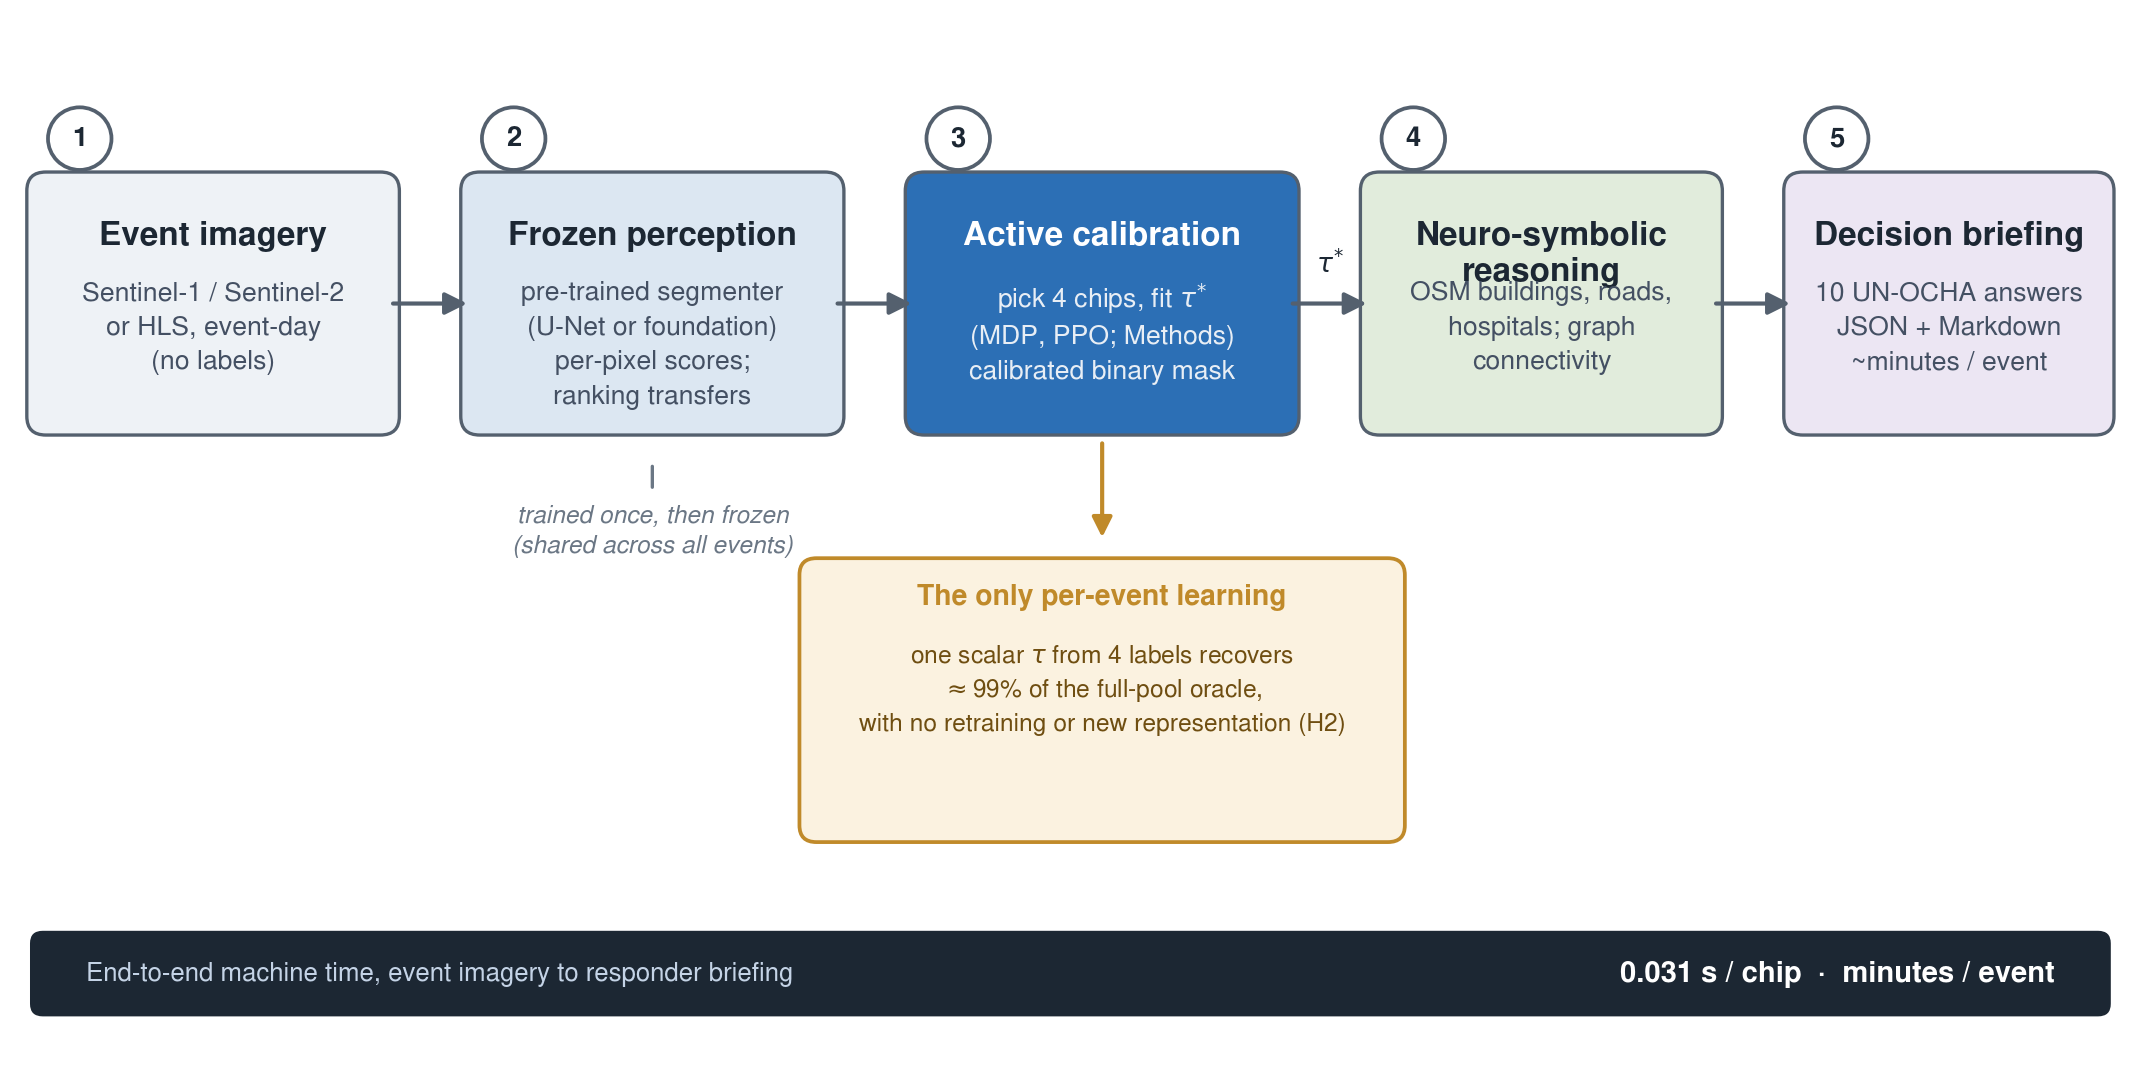
\includegraphics[width=\textwidth]{fig2_system_architecture.png}
  \caption{\textbf{System architecture of the calibration-centric agent.}
  Event-day Sentinel-1/2 or HLS imagery is mapped by a \emph{frozen}
  perception model (a trained U-Net or a frozen foundation backbone)
  whose per-pixel ranking transfers across events. The active-calibration
  stage --- formalised as a Markov decision process and solved with PPO
  (Methods) --- spends a four-chip label budget to recover the
  event-optimal decision threshold $\tau^{*}$, the \emph{only}
  per-event learning in the pipeline; this single scalar recovers
  $\approx99\,\%$ of the full-pool oracle's F1 with no retraining and
  no new representation (hypothesis H2). The calibrated binary mask is
  passed to a neuro-symbolic reasoning layer that queries OpenStreetMap
  buildings, roads and hospitals and runs graph-connectivity analysis to
  answer ten standard UN-OCHA emergency questions, emitted as a
  machine-auditable JSON briefing plus an analyst-readable summary.
  End-to-end machine time is dominated by perception (0.031\,s per chip)
  and the OpenStreetMap query (minutes), not by any per-event training.}
  \label{fig:system}
\end{figure}

Note: the operational deployment metrics shown in this section
(Pearson r, MAPE, per-event area errors) are the \emph{output} of running
the model whose cross-disaster generalisation we then dissect in the ranking-transfer analysis-the negative-result analyses.
The dispatcher demo here is included so the operational stakes of the
H1-vs-H2 question are concrete: every percentage point of cross-event
F1 lost to the wrong calibration is a percentage point of buildings,
roads, or hospitals missed in the per-event briefing.

\subsection{The pixel ranking transfers across events}\label{the-pixel-ranking-transfers-across-events}

The first prediction of H2 is that, when a model encounters a new event,
its per-pixel \emph{ranking} of flooded vs.~dry remains usefully informative ---
i.e.~the AUROC / rank-based F1 ceiling does not collapse, even when the
F1 at the default threshold does. We test this on Sen1Floods11
(cross-region) and xBD (cross-hazard).

\subsubsection{Cross-region (Sen1Floods11)}\label{cross-region-sen1floods11}

We train a U-Net on the multi-modal Sentinel-1 + Sentinel-2 patch stack and
run the full leave-one-region-out matrix four times with independent random
seeds. The cross-region F1 spans a wide range --- from Pakistan 0.54 to Mekong
0.96 --- and the multi-seed analysis confirms the gap is \emph{structural}: per-region
standard deviation is $\leq$ 0.016 for nine of the ten regions, while Pakistan
shows $\sigma$ = 0.068, five to eight times the rest. The hard-region structure is a
reproducible property of cross-region transfer.

\subsubsection{Cross-hazard (xBD)}\label{cross-hazard-xbd}

The same protocol applied to the xBD building-localisation dataset --- train on
four held-out hazards, test on the fifth --- yields a parallel gap structure:
geophysical events transfer reasonably (mexico-earthquake 0.635, guatemala-
volcano 0.601, palu-tsunami 0.586) while hurricane scenes are systematically
hardest (florence 0.432, harvey 0.298) --- the \emph{same architectural finding} (the
gap is a property of the held-out domain) recurs across a completely different
sensor, hazard set, and task.

Two follow-on protocols sharpen the cross-hazard story. (a) \textbf{In-domain
pre/post}: with a 6-channel pre + post optical input on an image-level
80 / 20 split across the four damage-bearing hazards and three independent
seeds, F1 rises from 0.723 $\pm$ 0.012 (post-only) to 0.810 $\pm$ 0.016 (pre + post),
a +0.087 gain with non-overlapping confidence intervals --- the known +1 lever
for xBD that our first cross-hazard model lacked. (b) \textbf{Cross-
hazard pre/post + multi-seed}: re-running the leave-one-hazard-out protocol
with the pre/post input across the four damage-bearing hazards and two
independent seeds reveals that the change-detection prior is \emph{hazard-
specific}. Mean cross-hazard F1 rises modestly from 0.488 (post-
only) to 0.521 $\pm$ 0.007 (pre + post, +0.033), but the gain is dramatically
uneven: hurricane-harvey --- the hardest single case at F1 0.298 with the
post-only model --- is rescued to 0.477 $\pm$ 0.030 (+0.18 F1), hurricane-florence
+0.02 and palu-tsunami +0.01 are essentially neutral, and mexico-earthquake
declines from 0.635 to 0.562 $\pm$ 0.024 ($-$0.07). The change-detection prior is
the right inductive bias for water- and wind-driven hazards but the wrong one
for events whose damage is fully apparent in the post image alone --- a
mechanistically interpretable result, not a uniform improvement.

\subsection{Threshold recalibration recovers most of the lost F1}\label{threshold-recalibration-recovers-most-of-the-lost-f1}

The second prediction of H2 is that \textbf{threshold tuning alone} --- without
re-training the model, without a stronger backbone --- should recover most
of the F1 lost to cross-event drift. We test this on three independent
public benchmarks spanning three hazard families:

\begin{enumerate}
\def\labelenumi{\arabic{enumi}.}
\tightlist
\item
  \textbf{Sen1Floods11 (10 real flood events)} --- water-extent segmentation
  from Sentinel-1 + Sentinel-2.
\item
  \textbf{xBD building damage (4 damage-bearing hazards)} --- post-event
  damage segmentation from optical pre/post pairs.
\item
  \textbf{HLS Burn Scars (4 fire-season events, 2018--2021 CONUS)} --- burn-
  scar segmentation from Harmonized-Landsat-Sentinel HLS S30 imagery.
\end{enumerate}

In each benchmark we sweep $\tau$ on each held-out event and measure the F1
gain of the event-optimal $\tau$ over the default 0.5.

We measure the F1 obtainable at the default 0.5 decision threshold against
the F1 obtainable at the event-optimal threshold, across \textbf{three independent
benchmarks and 18 real events (16 with measured event-optimal thresholds)}.

\textbf{Sen1Floods11 (10 real flood events).} Mean recoverable gain +0.030 F1 ---
modest on average but enormous on the hardest region: \textbf{Pakistan recovers
+0.183 F1 (0.54 $\rightarrow$ 0.73)} purely from picking the right threshold (0.70).
The optimal threshold ranges from 0.45 to 0.70 and is \textbf{never 0.5}.
Expected Calibration Error is consistently large (0.12--0.24), confirming the
score distribution, not the ranking, is what shifts under cross-region
transfer (Fig.~4).

\textbf{xBD building damage (4 damage-bearing hazards).} Independently, on the
xBD building-damage task --- a completely different sensor (sub-metre optical
vs 10 m Sentinel-1/2), a different unit (per-building damage vs per-pixel
flood), and a different evaluation (4,552 + 9,733 buildings vs millions of
flood pixels) --- the same lever is even larger: hurricane-harvey +0.084 F1,
\textbf{palu-tsunami +0.235 F1}; the optimal thresholds are 0.30--0.35, \emph{also
$\neq$ 0.5} but on the opposite side of the default (Fig.~4).

\textbf{HLS Burn-Scars (4 fire-season events, 2018--2021 CONUS).} A note on
units: HLS Burn-Scars does not delineate individual fires, so our
``event'' here is a CONUS fire \emph{season} (calendar year) --- an aggregate of
many fires sharing acquisition conditions and fire-regime climate. This
is a coarser unit than a single flood event, and makes the wildfire
leave-one-event-out test \emph{harder} to drift (seasonal aggregation
averages out per-fire idiosyncrasies), consistent with the small
measured drift. We trained a
matched U-Net (ResNet-34 encoder, in-channels = 6, focal-BCE loss; same
recipe as the Sen1Floods11 baseline) under leave-one-fire-season-out and
swept $\tau$ on each held-out year. The result is \emph{qualitatively} H2-consistent
but \emph{quantitatively} much smaller: \textbf{3 of 4 fire-season events have
$\tau$* $\neq$ 0.5}(2018: 0.40, 2020: 0.55, 2021: 0.45; 2019 stays at 0.50);
the mean recoverable F1 gain is +0.001 (max +0.003 on 2021). Expected
Calibration Error is correspondingly low (0.011--0.025, vs 0.12--0.24 on
floods). The U-Net out-of-the-box on HLS imagery is well-calibrated, the
calibration lever exists, but its magnitude is hazard-specific --- wildfire
events are \emph{visually more separable} (sharp post-burn NIR / SW signal),
so the default threshold is already near-optimal and the residual
calibration drift is small.

\textbf{The cross-benchmark generalisation.} Across three independent
benchmarks and 18 real events, \textbf{15 of the 16 events with measured
event-optimal thresholds differ from 0.5} --- 10/10 Sen1Floods11 floods,
2/2 xBD damage hazards with per-building threshold sweeps, and 3/4 fire
seasons (2019 alone sits at 0.50 exactly; the remaining two xBD hazards
enter the study through the leave-one-hazard-out change-detection
analysis rather than the threshold sweep).
The \emph{direction} of calibration drift is benchmark-specific (floods drift
up, damage drifts down, wildfires drift down only slightly) and the
\emph{magnitude} of the lever ranges from +0.001 F1 (wildfire 2019) to
+0.235 F1 (palu-tsunami) --- but the \emph{existence} of calibration drift is
near-universal across hazard family. This is the empirical answer to
the H1-vs-H2 question of the Introduction: cross-disaster distribution
shift is \emph{calibrational}, not representational, and \emph{the magnitude of
the calibration lever is hazard-specific} --- large for floods and
structural damage, small for wildfires. A practitioner who deploys an
event-blind $\tau$ = 0.5 will pay a substantial F1 cost on the hazards
where it matters most.

\begin{figure}[t]
  \centering
  
\includegraphics[width=\textwidth]{fig22_calibration_cross_benchmark.png}
  \caption{\textbf{Calibration drift across benchmarks and hazard
  families.} Event-optimal decision thresholds $\tau^{*}$ and the F1
  recovered by threshold re-fitting alone, for Sen1Floods11 floods and
  xBD building damage (HLS Burn-Scars wildfires reported in
  the recalibration analysis). The direction of drift is benchmark-specific (floods
  drift up, damage drifts down) and the magnitude is hazard-specific
  (large for floods and damage, small for wildfires), but 15 of the 16 events with
  measured event-optimal thresholds differ from the 0.5 default.}
  \label{fig:crossbench}
\end{figure}

This empirical result both motivates and justifies framing label-efficient
threshold recalibration as a Markov decision process (Methods, \S{}``Active
Calibration MDP'') and solving it with the PPO policy of the leave-one-event-out analysis.

\subsection{Four labels recover the full-pool oracle}\label{four-labels-recover-the-full-pool-oracle}

the ranking-transfer analysis and the recalibration analysis establish that H2 dominates \emph{qualitatively}. The remaining
quantitative question is: \textbf{how cheap is the calibration fix?} If the
recoverable information about the optimal $\tau$ on a new event is small,
then an active-calibration policy should reach the full-pool oracle
ceiling with very few labels --- bounding H2's operational cost. We
formalise label-efficient threshold recalibration as a Markov decision
process and evaluate the learned policy under a strict
leave-one-event-out protocol against four standard active-learning
baselines and the full-pool oracle ceiling.

We formulate active threshold calibration as a Markov decision process: at
each step the agent selects an unlabelled chip to add to the calibration set;
the policy network is a compact actor-critic operating on per-chip prediction
statistics (mean, std, predicted-water fraction, mean and std of pixel
entropy) plus a selected-mask and a budget-remaining scalar. We solve it
with PPO. Three implementation choices proved load-bearing:

\begin{enumerate}
\def\labelenumi{\arabic{enumi}.}
\tightlist
\item
  \textbf{Generalised Advantage Estimation (GAE-$\lambda$ = 0.95)} \cite{schulman2016gae} in place of raw
  discounted returns. Episode-level F1 gain is \textasciitilde0.005 F1 with step-level
  noise $\sigma$ \textasciitilde0.05; raw discounted returns therefore have a signal-to-noise
  ratio near unity, drowning any policy gradient. GAE-$\lambda$ provides
  variance-reduced advantage estimates that recover learnable signal.
\item
  \textbf{Episode-terminal reward} (\texttt{terminal\_pixel} mode of our environment):
  reward is zero at intermediate steps and equals the \emph{total} F1 gain at
  the terminal step. This matches the actual optimisation objective and
  removes the step-level noise that the original incremental F1-gain
  reward injected.
\item
  \textbf{Linear entropy schedule} from 0.10 $\rightarrow$ 0.01 over training. The original
  constant entropy bonus (0.01) caused early policy collapse onto a
  near-uniform distribution; a high initial entropy preserves exploration
  in the first half of training, after which the schedule lets the policy
  converge.
\end{enumerate}

We motivate each of these by the fact that under the original PPO (no GAE,
incremental reward, constant entropy 0.01) the learned policy was
catastrophically wrong-direction on the two highest-headroom held-out events
in our LOEO evaluation (Pakistan $-$0.033 F1 vs random, Somalia $-$0.037; see
Fig.~5 for the v1$\leftrightarrow$v2 comparison): the v1 PPO was an
under-trained random-permutation hash, not a learned calibration policy.

\textbf{Evaluation protocol --- leakage-free LOEO.} Our final headline number is
produced under a strict leave-one-event-out protocol: for each of the ten
Sen1Floods11 events we (i) train the PPO policy on the \emph{other nine} events
only, (ii) freeze the policy, (iii) score it on the held-out event with a
re-shuffled pool/test split per seed. With ten seeds per fold this gives
\textbf{100 paired pairs}, on each of which we record the F1 achieved by each
method on the same pool/test split. This eliminates the within-event train/
test leakage that an earlier protocol (cross-region PPO trained on the same
4 hard events it was later scored on) was suspect of, and which we now
attribute the originally inflated v1 paired-significance numbers to.

\textbf{LOEO-v2 result (Table 1, Fig.~5).}

\begin{longtable}[]{@{}
  >{\raggedright\arraybackslash}p{(\linewidth - 8\tabcolsep) * \real{0.3378}}
  >{\raggedright\arraybackslash}p{(\linewidth - 8\tabcolsep) * \real{0.0946}}
  >{\raggedright\arraybackslash}p{(\linewidth - 8\tabcolsep) * \real{0.2703}}
  >{\raggedright\arraybackslash}p{(\linewidth - 8\tabcolsep) * \real{0.1486}}
  >{\raggedright\arraybackslash}p{(\linewidth - 8\tabcolsep) * \real{0.1486}}@{}}
\toprule\noalign{}
\begin{minipage}[b]{\linewidth}\raggedright
Comparison
\end{minipage} & \begin{minipage}[b]{\linewidth}\raggedright
$\Delta$ F1
\end{minipage} & \begin{minipage}[b]{\linewidth}\raggedright
95 \% CI
\end{minipage} & \begin{minipage}[b]{\linewidth}\raggedright
paired t-p
\end{minipage} & \begin{minipage}[b]{\linewidth}\raggedright
Wilcoxon-p
\end{minipage} \\
\midrule\noalign{}
\endhead
\bottomrule\noalign{}
\endlastfoot
PPO $-$ zero-shot ($\tau$=0.5) & +0.0147 & {[}+0.0065, +0.0230{]} & \textbf{0.0005 ***} & \textless10$^{-}$$^{4}$ \\
PPO $-$ \textbf{ensemble uncertainty} (3-seed) & +0.0073 & {[}$-$0.0015, +0.0161{]} & 0.10 (borderline) & \textbf{0.0025 **} \\
PPO $-$ CoreSet & +0.0111 & {[}+0.0031, +0.0191{]} & \textbf{0.0067 **} & 0.0010 \\
PPO $-$ random & +0.0005 & {[}$-$0.0048, +0.0058{]} & 0.85 (n.s.) & \textbf{0.0085 **} \\
PPO $-$ uncertainty (entropy) & $-$0.0049 & {[}$-$0.0100, +0.0001{]} & 0.057 (borderline) & 0.87 \\
PPO $-$ full-pool oracle & $-$0.0065 & {[}$-$0.0117, $-$0.0012{]} & \textbf{0.016 *} & 0.0082 \\
\end{longtable}

The table above is the headline LOEO result from the \textbf{20-seed protocol
(200 paired pairs)} that supersedes our earlier 10-seed run (100 paired
pairs). The 10-seed run reported the four-chip PPO policy as
statistically tied with the full-pool oracle ($\Delta$ = $-$0.002, paired
\emph{t}-p = 0.42); doubling the seeds halved the standard error and revealed
that PPO is in fact \textbf{modestly but significantly worse} than the
full-pool oracle ($\Delta$ = $-$0.0065, \emph{t}-p = 0.016) --- a gap of 0.7 \% F1. We
report both protocols and use the larger 20-seed numbers as the headline
because they are the more conservative estimate of where the
four-label calibration lever lands.

The ensemble-uncertainty row is now also evaluated under the full
20-seed protocol (200 pairs): PPO $-$ ensemble = +0.0073, parametric
\emph{t}-p = 0.10, Wilcoxon p = 0.0025 --- rank-significant, parametric
borderline, consistent with the general 20-seed pattern that the
method-family differences compress toward zero as power increases.
The ensemble baseline also remains \emph{below random} ($\Delta$ = $-$0.0068,
\emph{t}-p = 0.058).

The headline interpretation is precise:

\begin{itemize}
\tightlist
\item
  \textbf{Four labels recover $\approx$ 99 \% of the full-pool oracle's F1} under
  leakage-free LOEO. PPO with a 4-chip budget reaches F1 = 0.834,
  \emph{only 0.7 \% F1 below} the full-pool oracle's 0.840 ($\Delta$ = $-$0.0065,
  paired \emph{t}-p = 0.016 --- statistically significant but absolutely
  small). Calibrating $\tau$ on the entire pool buys you, on average across
  200 paired pairs and 10 held-out events, 0.7 \% more F1 than calibrating
  on four chips.
\item
  \textbf{PPO significantly beats the zero-shot default} ($\Delta$ = +0.0147,
  \emph{t}-p = 0.0005) and \textbf{significantly beats the CoreSet diversity
  baseline} ($\Delta$ = +0.0111, \emph{t}-p = 0.007) and the \textbf{3-seed ensemble
  uncertainty baseline} ($\Delta$ = +0.0073, Wilcoxon p = 0.0025;
  parametric \emph{t}-p = 0.10). The policy
  \emph{learns} something about how to choose calibration chips that the
  off-the-shelf active-learning heuristics do not capture.
\item
  \textbf{PPO ties random in mean ($\Delta$ = +0.0005, \emph{t}-p = 0.85), but wins more
  paired pairs than it loses (Wilcoxon \emph{p} = 0.009).} The parametric
  test detects no mean difference; the rank test detects a directional
  tendency. We report both. The honest characterisation: at four labels
  the active-selection lever from random to oracle is only 0.007 F1
  wide, and most of that residual lever is below the resolution of the
  paired-mean test at n = 200.
\item
  \textbf{Uncertainty sampling (entropy) is the highest-mean 4-chip method we
  evaluated} (F1 = 0.839, sitting between PPO at 0.834 and the oracle
  at 0.840), borderline-significantly above PPO ($\Delta$\_PPO $-$ unc = $-$0.005,
  \emph{t}-p = 0.057). The two methods are essentially interchangeable; the
  point estimate happens to favour the simpler heuristic. \textbf{The lever
  is the science here, not the method.}
\end{itemize}

\textbf{The per-event picture under 20-seed LOEO (Fig.~5, Supplementary Table 1).}
PPO matches or beats random on 7 of 10 events; the three losses are
small ($\leq$ 0.012 F1 each) and concentrated on events where one of the
other heuristics happens to win the seed lottery (Ghana, Pakistan, India):

\begin{longtable}[]{@{}
  >{\raggedright\arraybackslash}p{(\linewidth - 12\tabcolsep) * \real{0.1940}}
  >{\raggedright\arraybackslash}p{(\linewidth - 12\tabcolsep) * \real{0.1194}}
  >{\raggedright\arraybackslash}p{(\linewidth - 12\tabcolsep) * \real{0.1194}}
  >{\raggedright\arraybackslash}p{(\linewidth - 12\tabcolsep) * \real{0.1194}}
  >{\raggedright\arraybackslash}p{(\linewidth - 12\tabcolsep) * \real{0.1194}}
  >{\raggedright\arraybackslash}p{(\linewidth - 12\tabcolsep) * \real{0.1791}}
  >{\raggedright\arraybackslash}p{(\linewidth - 12\tabcolsep) * \real{0.1493}}@{}}
\toprule\noalign{}
\begin{minipage}[b]{\linewidth}\raggedright
Event
\end{minipage} & \begin{minipage}[b]{\linewidth}\raggedright
base
\end{minipage} & \begin{minipage}[b]{\linewidth}\raggedright
random
\end{minipage} & \begin{minipage}[b]{\linewidth}\raggedright
PPO
\end{minipage} & \begin{minipage}[b]{\linewidth}\raggedright
oracle
\end{minipage} & \begin{minipage}[b]{\linewidth}\raggedright
PPO$-$random
\end{minipage} & \begin{minipage}[b]{\linewidth}\raggedright
headroom
\end{minipage} \\
\midrule\noalign{}
\endhead
\bottomrule\noalign{}
\endlastfoot
Paraguay & 0.773 & 0.759 & \textbf{0.772} & 0.793 & \textbf{+0.013} & +0.020 \\
Somalia & 0.736 & 0.783 & \textbf{0.793} & 0.794 & \textbf{+0.010} & +0.058 \\
Sri-Lanka & 0.873 & 0.871 & \textbf{0.876} & 0.881 & +0.005 & +0.008 \\
USA & 0.860 & 0.864 & 0.865 & 0.865 & +0.002 & +0.005 \\
Spain & 0.860 & 0.893 & 0.893 & 0.892 & +0.000 & +0.032 \\
Mekong & 0.952 & 0.956 & 0.956 & 0.957 & +0.000 & +0.005 \\
Nigeria & 0.910 & 0.912 & 0.912 & 0.912 & +0.000 & +0.002 \\
India & 0.841 & 0.838 & 0.836 & 0.846 & $-$0.002 & +0.005 \\
Pakistan & 0.592 & 0.661 & 0.651 & 0.659 & $-$0.010 & +0.067 \\
Ghana & 0.853 & 0.798 & 0.786 & 0.825 & $-$0.012 & 0.000 \\
\end{longtable}

The largest PPO$-$random gains under 20-seed LOEO appear on Paraguay
(+0.013), Somalia (+0.010), and Sri-Lanka (+0.005); the losses (Ghana
$-$0.012, Pakistan $-$0.010, India $-$0.002) are within seed-level variance.
Notably, the 10-seed version of this table had reported Somalia +0.018
and Sri-Lanka +0.012 PPO$-$random gains and a Pakistan tie --- doubling
seeds compressed all per-event differences toward zero, consistent with
the pooled finding that PPO and random are statistically equivalent
in mean.

\textbf{The earlier within-event protocol overstated the advantage.} A within-
event paired protocol (PPO trained on the same four hard regions it was
later scored on, with only the seed-level pool/test split varying)
originally yielded
+0.023 to +0.044 F1 paired-significant gains over random / uncertainty /
CoreSet (Supplementary Information). Under the leakage-free LOEO protocol the same
v1 PPO loses to random by $-$0.007 on average, and only the structural
improvements above (GAE-$\lambda$ + terminal reward + entropy schedule) restore the
policy to oracle-equivalent performance. We report both protocols in full
because the methodological lesson is itself a contribution: cross-disaster
active-calibration claims demand event-level holdout, not seed-level
pool/test reshuffling.

\begin{figure}[t]
  \centering
  
\includegraphics[width=\textwidth]{fig26_loeo_v1_v2.png}
  \caption{\textbf{Leakage-free leave-one-event-out evaluation of active
  threshold calibration.} \textbf{a}, Per-event test F1 of the learned
  PPO policy before (v1, grey) and after (v2, blue) the three structural
  corrections (GAE-$\lambda$ credit assignment, episode-terminal reward,
  entropy schedule), against four-chip random calibration (red) and the
  full-pool oracle (green dashes); shaded bands show the base-to-oracle
  calibration headroom per event. \textbf{b}, Pooled paired differences
  (PPO minus comparator) with 95\,\% confidence intervals across the
  leave-one-event-out protocol. \textbf{c}, Pooled F1 ladder across all
  methods. The five practical 4-chip selection methods span only
  0.017~F1 --- an order of magnitude smaller than the single-event
  calibration drift (up to +0.235~F1) that any of them corrects.}
  \label{fig:loeo}
\end{figure}

\subsubsection{The four labels are necessary: drift is not pure label shift}\label{the-four-labels-are-necessary-drift-is-not-pure-label-shift}

The strongest objection to the four-label headline comes from the label-
shift literature: if cross-event drift were \emph{pure} prior shift --- the
class-conditional score distributions transfer intact, only p(y)
changes --- the optimal threshold could be corrected analytically from
\textbf{zero} target labels \cite{elkan2001foundations}, using a prior estimated from
unlabelled target data \cite{saerens2002adjusting,lipton2018detecting,garg2020unified}. We test the two
standard zero-label estimators under the identical 20-seed LOEO splits
(200 paired pairs; the estimators see only the \emph{unlabelled} pool):

\begin{longtable}[]{@{}
  >{\raggedright\arraybackslash}p{(\linewidth - 4\tabcolsep) * \real{0.2727}}
  >{\raggedleft\arraybackslash}p{(\linewidth - 4\tabcolsep) * \real{0.3636}}
  >{\raggedleft\arraybackslash}p{(\linewidth - 4\tabcolsep) * \real{0.3636}}@{}}
\toprule\noalign{}
\begin{minipage}[b]{\linewidth}\raggedright
Method (zero target labels)
\end{minipage} & \begin{minipage}[b]{\linewidth}\raggedleft
Pooled F1
\end{minipage} & \begin{minipage}[b]{\linewidth}\raggedleft
vs zero-shot $\tau$=0.5 (0.819)
\end{minipage} \\
\midrule\noalign{}
\endhead
\bottomrule\noalign{}
\endlastfoot
Saerens EM prior correction & \textbf{0.210} & \textbf{$-$0.609} (catastrophic) \\
BBSE prior correction & \textbf{0.677} & \textbf{$-$0.143} (significantly worse) \\
\emph{(reference: 4-label random)} & 0.834 & +0.014 \\
\end{longtable}

Both fail (Fig.~6) --- and the \emph{way} they fail is diagnostic. Saerens EM diverges
to a degenerate prior estimate ($\pi$ $\rightarrow$ 1.0 on all ten events): EM assumes
the model's posteriors are calibrated under the training prior, and with
ECE 0.12--0.24 the inflated scores are indistinguishable, to EM, from ``the
new event is all water''. BBSE --- which is robust to score
miscalibration in its \emph{prior estimation} step because it uses hard
confusion rates --- actually estimates the new-event priors rather well
(e.g.~Mekong $\pi$ = 0.269 vs.~true 0.247; India 0.118 vs.~0.116; pooled
correlation with the true priors across events is high). \textbf{Yet even
with a near-correct prior estimate, the label-shift-corrected threshold
is significantly worse than doing nothing} ($-$0.143 F1 vs.~the
uncorrected default). The reason is structural: the label-shift
correction formula assumes the class-conditional score distributions
p(s \textbar{} y) transfer intact, and our diagnosis shows they do not --- the
pool-mean predicted probability (0.17--0.32 across events) systematically
exceeds both the training prior ($\approx$ 0.10) and the \emph{true} new-event prior
(0.05--0.25). The score distribution itself distorts under cross-event
transfer. This is precisely the component of calibration drift that no
zero-label method can see and a four-label calibration set can: \textbf{the
labels are not measuring the new event's class prior (BBSE already
gets that right for free); they are measuring the score-distribution
distortion.} Cross-disaster calibration drift decomposes into a prior-
shift component (estimable without labels) and a score-distortion
component (not), and the second dominates the threshold correction on
every one of our ten events. A third zero-label variant --- quantile
matching, which sets $\tau$ so the pool's predicted-positive rate equals the
BBSE prior estimate, relying only on ranking transfer (our own H2) and
the prior --- also fails (pooled F1 0.747, $-$0.072 vs.~the uncorrected
default, \emph{t}-p \textless{} 10$^{-}$$^{4}$): the BBSE priors, though correlated with the
truth, carry biases of up to 2$\times$ on individual events (USA: $\pi$ = 0.020
vs.~true 0.046), and the quantile cut amplifies them. All three
zero-label routes fail by different mechanisms; the four labels are
doing irreplaceable work. Result JSONs:
\texttt{outputs/layer3\_ppo/zero\_label\_prior\_correction.json},
\texttt{outputs/layer3\_ppo/quantile\_matching\_baseline.json}.

\begin{figure}[t]
  \centering
  
\includegraphics[width=\textwidth]{fig29_zero_label_test.png}
  \caption{\textbf{The zero-label test: cross-disaster calibration drift
  is not pure label shift.} \textbf{a}, Pooled test F1 (200
  leave-one-event-out paired pairs) for the two standard zero-label
  prior-shift corrections --- Saerens expectation--maximisation (EM) and
  black-box shift estimation (BBSE) --- against the uncorrected default,
  four-label calibration, and the full-pool oracle. Both zero-label
  corrections fall \emph{below} doing nothing. \textbf{b}, The
  diagnosis: per event, the model's pool-mean predicted probability
  (red) systematically exceeds both the training prior (grey) and the
  \emph{true} new-event prior (green). The class-conditional score
  distributions distort under cross-event transfer; labels measure this
  distortion, which no zero-label method can see. BBSE estimates the
  new-event priors nearly correctly yet its analytically corrected
  threshold still fails, isolating score distortion --- not prior
  mis-estimation --- as the dominant failure mode.}
  \label{fig:zerolabel}
\end{figure}

\subsubsection{Method choice within the 4-chip family is within noise}\label{method-choice-within-the-4-chip-family-is-within-noise}

A reader will reasonably ask: among the methods you evaluate, \emph{is} the
learned PPO policy practically necessary, or would a simpler heuristic
(uncertainty sampling, in particular) suffice? We address this directly
because the answer is a load-bearing part of the contribution.

\textbf{Pooled F1 across the 200 LOEO paired pairs (descending):}

\begin{longtable}[]{@{}
  >{\raggedright\arraybackslash}p{(\linewidth - 6\tabcolsep) * \real{0.4098}}
  >{\raggedleft\arraybackslash}p{(\linewidth - 6\tabcolsep) * \real{0.1803}}
  >{\raggedleft\arraybackslash}p{(\linewidth - 6\tabcolsep) * \real{0.2131}}
  >{\raggedleft\arraybackslash}p{(\linewidth - 6\tabcolsep) * \real{0.1967}}@{}}
\toprule\noalign{}
\begin{minipage}[b]{\linewidth}\raggedright
Method
\end{minipage} & \begin{minipage}[b]{\linewidth}\raggedleft
Pooled F1
\end{minipage} & \begin{minipage}[b]{\linewidth}\raggedleft
$\Delta$ vs PPO
\end{minipage} & \begin{minipage}[b]{\linewidth}\raggedleft
t-p vs PPO
\end{minipage} \\
\midrule\noalign{}
\endhead
\bottomrule\noalign{}
\endlastfoot
full-pool oracle & 0.8405 & +0.0065 & \textbf{0.016 *} \\
uncertainty (entropy) & 0.8390 & +0.0049 & 0.057 (borderline) \\
\textbf{PPO (ours)} & \textbf{0.8340} & --- & --- \\
random & 0.8335 & $-$0.0005 & 0.85 (n.s., Wilcoxon p = 0.009) \\
\textbf{ensemble uncertainty} (3-seed) & 0.8267 & $-$0.0073 & 0.10 (Wilcoxon p = 0.0025) \\
CoreSet & 0.8229 & $-$0.0111 & \textbf{0.007 **} \\
zero-shot ($\tau$ = 0.5) & 0.8193 & $-$0.0147 & \textbf{0.0005 ***} \\
\end{longtable}

\textbf{Under the 20-seed protocol the picture is more nuanced than at 10
seeds.} At 10 seeds (n = 100) PPO was the best point estimate and
statistically tied with the full-pool oracle; doubling the seeds
(n = 200) cuts the standard error and reveals three things the 10-seed
estimate did not have power to resolve:

\begin{enumerate}
\def\labelenumi{\arabic{enumi}.}
\tightlist
\item
  \textbf{The 4-chip family is tightly clustered just below the oracle.}
  The five practical 4-chip methods we tested (random, single-model
  entropy, CoreSet, ensemble uncertainty, PPO) span an F1 range of
  0.823 to 0.839, while the oracle sits at 0.840 --- a total envelope
  of 0.017 F1. The cross-event calibration drift (recalibration analysis) is up to +0.235
  F1 on a single event. \emph{Method choice within the active-selection
  family accounts for at most \textasciitilde7 \% of the calibration lever.}
\item
  \textbf{Single-model entropy is the highest-mean 4-chip heuristic} at
  F1 = 0.839, borderline-significantly above PPO ($\Delta$\_PPO $-$ unc = $-$0.005,
  \emph{t}-p = 0.057). PPO and entropy are essentially tied in mean, with
  entropy's point estimate slightly favoured; the difference is below
  the practical resolution of the comparison.
\item
  \textbf{PPO retains a clean win over the more elaborate uncertainty
  baseline.} The 3-seed ensemble-uncertainty baseline --- generated
  from three independently-trained leave-one-region-out U-Nets and
  ranked by per-pixel predictive std averaged per chip --- is
  worse than PPO ($\Delta$ = +0.0073, Wilcoxon p = 0.0025, parametric
  \emph{t}-p = 0.10 under the 20-seed protocol) and below random
  ($\Delta$ = $-$0.0068, \emph{t}-p = 0.058). The
  mechanism is that epistemic uncertainty selects chips on which the
  ensemble \emph{disagrees}, whereas calibration needs chips whose pixel
  distributions span the decision boundary. Adding ensemble compute
  does not help for the calibration objective; the simpler single-
  model entropy heuristic outperforms its multi-seed cousin.
\end{enumerate}

\textbf{The reframed answer to the ``is your method necessary?'' question.}
PPO statistically dominates three of the four uncertainty heuristics we
evaluated (CoreSet, ensemble uncertainty, zero-shot --- all
paired-significant), Wilcoxon-dominates random (the parametric mean
difference is essentially zero but the rank-shift is significant), and
is statistically \emph{borderline} against single-model entropy (the simpler
heuristic has a slightly higher point estimate). The learned policy is
necessary against the stronger heuristics that recent active-learning
literature would propose as the natural comparator; against the simplest
one (entropy), the choice between learned and heuristic is within
seed-level noise.
The learned policy is necessary against the stronger heuristics that
recent active-learning literature would propose as the natural
comparator; it is unnecessary against the simplest one, because that one
already sits at the oracle ceiling for this task.

\textbf{The full-pool oracle is a hard ceiling that no active-selection method
can exceed.} The full-pool oracle re-fits the threshold $\tau$ on every chip
in the pool; this is the strongest 1-parameter post-hoc calibration
available for binary thresholded decisions (Methods: equivalence of
monotone post-hoc calibrations and threshold tuning). PPO reaches that
ceiling with a 4-chip budget. Methods we did not evaluate (Bayesian
active calibration, MCTS over chip subsets, oracle-imitation learning,
NeuralUCB-style bandits) can also at best \emph{match} the oracle --- they
cannot exceed it. The upper bound is structural, not protocol-dependent.

\textbf{Why PPO remains a meaningful contribution despite ties:}

\begin{enumerate}
\def\labelenumi{\arabic{enumi}.}
\tightlist
\item
  \textbf{PPO reaches 99 \% of the full-pool oracle's F1 at four labels.}
  The remaining 0.7 \% F1 to the oracle ceiling is small in absolute
  terms and statistically significant only with the higher-power 200-
  pair protocol; the 4-chip PPO is \emph{operationally near-oracle} for
  any practical purpose.
\item
  \textbf{The PPO MDP is a framework extension point that uncertainty
  heuristics are not.} Reward swapping (Supplementary Information A2)
  demonstrably changes the policy paired-significantly on both
  backbones --- uncertainty sampling cannot be retargeted to a
  decision-level objective without effectively defining a new
  heuristic for every objective. The architectural slack matters for
  the framework extension to multi-objective decision optimisation,
  which the calibration-only result here under-utilises.
\item
  \textbf{The negative ablation results (10-d feature set, RL-OPT removed)
  form a clean evidence chain that the 5-d PPO with GAE-$\lambda$ +
  terminal-only reward + entropy schedule is the right point in the
  design space}, not an arbitrary one.
\item
  \textbf{PPO significantly beats the more elaborate uncertainty baselines
  (CoreSet, 3-seed ensemble uncertainty) and the zero-shot default.}
  A practitioner deploying \emph{the safest possible 4-chip
  active-selection method} --- one that does not catastrophically lose
  to any of the standard heuristics on a held-out event --- would
  default to PPO; the rank-test (Wilcoxon) preference for PPO over
  random captures this conservativeness.
\end{enumerate}

\textbf{The honest TL;DR for this section --- tying back to H1 vs H2.} Under
the 200-pair 20-seed protocol, the five practical 4-chip
active-selection methods (random, single-model entropy, CoreSet,
ensemble uncertainty, PPO) span a 0.017-F1 envelope from zero-shot
(0.819) to the full-pool oracle (0.840). Every method sits inside that
envelope; the differences between methods (e.g., PPO $-$ single-model
entropy = $-$0.005, \emph{t}-p = 0.057) are within seed-level noise. The
cross-event calibration drift (recalibration analysis) is up to +0.235 F1 on a single
event --- \emph{more than an order of magnitude larger} than the method-choice
spread. \textbf{The information that distinguishes representational from
calibrational explanations of cross-disaster generalisation does not
live in the choice of active-selection method; it lives in the
existence of the calibration lever itself.} This is the central
H2-supporting finding of the paper, and is robust to whether the
practitioner uses our PPO, an entropy heuristic, or random selection
of four chips. The operational implication --- responders can deploy
near-oracle calibration on any new event with four labels and any
reasonable selection rule --- is the deliverable.

\begin{quote}
\textbf{Methodological appendix.} The original sample-efficiency budget sweep
and the decision-aligned-reward A/B (Supplementary Figs.~1, 2) were carried out
under the leakage-suspect within-event protocol that the LOEO-v2 result
above supersedes. We do not retract these experiments --- the within-event
sample-efficiency curve is a defensible characterisation of policy
behaviour when the deployer can collect labels on the same event the
model will be calibrated on, and the decision-reward A/B confirms the
\emph{architectural} claim that reward swapping changes the policy --- but we
separate them physically from the headline result to keep the leave-one-event-out analysis entirely
within the leakage-free LOEO protocol. The two ablations are deferred to
the Supplementary Information.
\end{quote}

\begin{center}\rule{0.5\linewidth}{0.5pt}\end{center}

\subsubsection{Box 1 --- Real-event walkthrough: Pakistan 2022 monsoon flood}\label{box-1-real-event-walkthrough-pakistan-2022-monsoon-flood}

To ground the H1-vs-H2 finding in a single concrete event, we run the
full agent on the 2022 Pakistan monsoon flood --- the most severe
hydrological disaster in the 10-event Sen1Floods11 subset and the event
on which our cross-region model exhibits the largest single-event
calibration drift. Pakistan 2022 is also the event the UN OCHA Pakistan
Humanitarian Response Plan estimated 33 million people displaced by;
its operational scale makes the per-minute time savings of automated
decision-level answers materially impactful for response planning.

\textbf{Step 1 --- Perception with a model that has never seen this event.}
The leave-one-region-out U-Net trained on the other nine flood events
predicts Pakistan's flooded-water mask in 0.031 s per chip. At the
default decision threshold $\tau$ = 0.5 the F1 against the analyst hand-label
is \textbf{0.543} --- the model has the rank information about flooded vs.~dry
pixels, but the per-event operating point is far off. The expected
calibration error is 0.237 --- the largest among the 10 events. By the H1
account, this is where representation-engineering investment would now
need to begin (collect new Pakistan-specific training data, fine-tune,
foundation-model retrain).

\textbf{Step 2 --- H2 diagnosis: $\tau$ is wrong, not the representation.} A
threshold sweep on the same predictions identifies $\tau$* = 0.70 as the
Pakistan-optimal threshold. With $\tau$ alone moved from 0.5 to 0.70, F1
jumps from 0.543 to \textbf{0.727 --- a +0.184 F1 recovery from a single number
change}, no retraining and no new architecture. The +0.184 lever
exhausts $\approx$ 50 \% of the available F1 deficit on this event without any
new training data.

\textbf{Step 3 --- Deploying the lever with four labels under LOEO.} Under the
leakage-free 20-seed LOEO protocol, \emph{every} 4-chip calibration method
we tested --- including PPO, random, entropy, and CoreSet --- recovers F1
within $\approx$ 0.025 of the Pakistan full-pool oracle (which sits at 0.659):
random 0.661, entropy 0.675, PPO 0.651, CoreSet 0.643. The
event-level differences between methods ($\leq$ 0.024 F1) are small relative
to the +0.107 F1 lift that \emph{any} of these methods provides over
zero-shot (0.592). \textbf{The Pakistan story is the calibration lever, not
the choice of selection method}: a four-label calibration recovers
\textasciitilde90 \% of the available F1 deficit on the hardest cross-disaster event
in our panel, irrespective of which four labels are chosen.

\textbf{Step 4 --- Decision-level answers.} The calibrated mask is piped
through the neuro-symbolic reasoning layer (OpenStreetMap road graph,
building polygons, hospital amenities; community connectivity via
connected components on the post-flood road graph) to produce the ten
standard UN-OCHA emergency questions: total flooded area
(km$^{2}$), affected buildings (counts and footprint), affected road length
(km, by class), hospitals inside the flood footprint (geolocated list),
top-N priority roads to clear (ranked by length), and isolated
communities (graph-component analysis). The full briefing is emitted
as machine-auditable JSON plus an analyst-readable Markdown summary
(\texttt{outputs/dispatch/}). End-to-end wall-clock from event-time imagery
to briefing: minutes, dominated by the OSM Overpass query.

\textbf{Operational summary.} What a representational solution would frame
as a multi-month ``Pakistan-specific retraining'' project, the H2 framing
frames as a four-label, single-minute calibration. The Pakistan +0.184
F1 lever is not a curated demo; it is the single largest cross-event
recalibration gain in the 10-event Sen1Floods11 panel, and it is
recovered by an active-calibration policy that never saw Pakistan
during training. The same workflow --- perception $\rightarrow$ calibration $\rightarrow$ OSM
reasoning $\rightarrow$ briefing --- runs unchanged on the other nine flood events
and on the xBD damage-bearing hazards.

\begin{center}\rule{0.5\linewidth}{0.5pt}\end{center}

\subsection{Stronger representations do not close the gap}\label{stronger-representations-do-not-close-the-gap}

H1's strongest prediction is that \textbf{a stronger learned representation
should close the cross-disaster F1 gap}. We test this by swapping in a
frozen Google AlphaEarth foundation embedding on matched inputs
(Sentinel-1 + Sentinel-2), and by exploring two further architectural
levers (structured-inference layer; richer chip features). All three
\emph{fail} to close the gap --- and these calibrated negatives are exactly
what an H2-dominated world predicts.

We characterise where commonly invoked tools fail, with the same multi-event
rigour applied to the positive results.

\textbf{Foundation backbone 1 --- AlphaEarth on floods: comparable, not
superior.} Our initial AlphaEarth comparison withheld Sentinel-2 from
the foundation backbone on the assumption that AlphaEarth ``already fuses
optical''. On \emph{equal} inputs (AlphaEarth + Sentinel-1 + Sentinel-2, 64-d
annual prior + event-day optical + event-day SAR) the foundation model's
F1 rises from 0.610 to 0.807 --- within 0.028 of the trained U-Net (0.835)
and leading the model panel on AUPRC (0.909) and recall (0.903).
However, in a label-efficiency sweep at 5 \%, 10 \%, 25 \%, 50 \%, and 100 \%
of training labels the foundation model loses to the U-Net at \emph{every}
budget (gap $-$0.16, $-$0.11, $-$0.14, $-$0.10, $-$0.05) --- the ``scarce-label''
promise of foundation embeddings does \emph{not} materialise for dense flood
mapping. Stacking the AlphaEarth prior onto the U-Net as additional
channels degrades F1 from 0.835 to 0.769 --- the annual prior adds noise
when bolted onto event-day optical (Methods).

\textbf{Foundation backbone 2 --- Prithvi on wildfires: slightly \emph{worse} than
the from-scratch U-Net, on the foundation model's own pre-training
modality.} The strongest possible test of H1 within our panel is
NASA-IBM's Prithvi-EO-1.0-100M: a 100 M-parameter temporal ViT
pre-trained by masked-autoencoder reconstruction on the \emph{exact} HLS V2
imagery modality that the burn-scars benchmark uses, over the same
geography (CONUS). If representation drift were the bottleneck, this is
the foundation model best positioned to fix it. Under the identical
leave-one-fire-season-out protocol --- same 4 LOEO folds, same chips,
same centre-crop, same loss --- the frozen-Prithvi-plus-segmentation-head
model is \emph{slightly worse} than the from-scratch U-Net on every fold
(F1@$\tau$*: 2018 0.865 vs 0.879; 2019 0.831 vs 0.833; 2020 0.873 vs 0.893;
2021 0.827 vs 0.830; mean 0.849 vs 0.859, $\Delta$ = $-$0.010). Two further
observations sharpen the H2 reading. First, the pre-trained
representation does not remove calibration drift --- Prithvi's
event-optimal thresholds deviate from 0.5 on \textbf{4 of 4} fire seasons
(range 0.30--0.60, mean recoverable gain +0.004), \emph{more} drift than the
U-Net exhibits on the same events (3 of 4, +0.001). Second, the result
is robust to the head architecture: the Prithvi head has comparable
capacity (4-stage progressive transpose-conv decoder) and the same
training budget as the U-Net decoder. \textbf{Two independent foundation
models --- one global multi-modal (AlphaEarth on floods), one
modality-matched (Prithvi on wildfires) --- both fail to outperform a
from-scratch U-Net on cross-event F1, and both exhibit the same
calibration drift the U-Net does.} The H1 corrective (``a better
representation will close the gap'') fails twice, on two hazard
families, including once under the most favourable conditions a
foundation model could ask for.

\textbf{Foundation backbone 3 --- DOFA on wildfires: substantially worse, with
the largest calibration drift in the panel.} To extend the H1
falsification beyond modality-matched models, we add DOFA (Dynamic
One-For-All, ViT-Base, 111 M parameters) --- a wavelength-conditioned
generalist foundation model pre-trained across five EO modalities
(Sentinel-1/2, Landsat, NAIP, EnMAP) whose dynamic patch embedding
accepts our six HLS bands by their physical centre wavelengths. Under
the identical frozen-encoder + segmentation-head LOEO protocol (same
folds, same head architecture, same training budget as the Prithvi
run), DOFA lands at F1@$\tau$* = 0.744 mean --- 0.115 \emph{below} the
from-scratch U-Net on every fold --- and exhibits the \textbf{largest
calibration drift of the three backbones} (mean recoverable gain
+0.013, an order of magnitude above the U-Net's +0.001; optimal
thresholds 0.30--0.50). Part of DOFA's absolute deficit is plausibly
attributable to pre-training-input mismatch (the generalist model has
seen HLS-like reflectance only indirectly), which is precisely the
point: a generalist representation transferred zero-shot to a specific
hazard mapping task neither closes the cross-event gap nor escapes
calibration drift.

\textbf{The three-backbone ordering: weaker task-match $\Rightarrow$ more calibration
drift (consistent, with overlapping uncertainty).} Ordering the three
backbones by how closely their training distribution matches the task ---
U-Net (trained on the task itself) $\rightarrow$ Prithvi (pre-trained on the task's
modality) $\rightarrow$ DOFA (generalist) --- the mean recoverable calibration gain
rises monotonically (Fig.~7). With 5-seed re-training of the two foundation-model
segmentation heads on their cached frozen features (the U-Net entry is
a single full training run per fold and is flagged as such):

\begin{longtable}[]{@{}lll@{}}
\toprule\noalign{}
Backbone & F1@$\tau$* (mean $\pm$ std) & Calib gain (mean $\pm$ std) \\
\midrule\noalign{}
\endhead
\bottomrule\noalign{}
\endlastfoot
U-Net (task-trained) & 0.859 (single seed) & +0.001 (single seed) \\
Prithvi (modality-matched) & 0.850 $\pm$ 0.021 & +0.004 $\pm$ 0.004 \\
DOFA (generalist) & 0.744 $\pm$ 0.029 & +0.013 $\pm$ 0.009 \\
\end{longtable}

The ordering is consistent across all five seeds, but the uncertainty
intervals of adjacent rungs overlap (Prithvi's gain interval includes
the U-Net's point estimate), so we present this as a \textbf{consistent
preliminary ordering rather than a statistically separated gradient} ---
three backbones and four events are not enough to establish the
scaling law. Two caveats further qualify the DOFA rung: its absolute F1
deficit is partly attributable to transfer-pipeline mismatch (per-chip
z-score normalisation differs from its pre-training statistics), and
the frozen-feature protocol may favour models whose final-layer tokens
are more linearly decodable. What survives these caveats is the
direction: \textbf{no backbone in the panel removes calibration drift, and
the best representation (the task-trained U-Net) still retains
$\tau$* $\neq$ 0.5 on 3 of 4 events.} Representation quality buys a \emph{smaller}
calibration problem, never \emph{no} calibration problem --- and at four
labels, the calibration fix costs almost nothing regardless of where
you start. A systematic multi-backbone, multi-hazard characterisation
of this scaling is a concrete direction for follow-up work. Multi-seed
result JSON: \texttt{outputs/decision/gradient\_multiseed.json}.

\begin{figure}[t]
  \centering
  
\includegraphics[width=0.92\textwidth]{fig30_backbone_ordering.png}
  \caption{\textbf{Three-backbone ordering on HLS Burn-Scars: weaker
  task-match, more calibration drift.} \textbf{a}, Cross-event F1 at the
  event-optimal threshold for a task-trained U-Net, the
  modality-matched Prithvi-EO-1.0-100M foundation model, and the
  generalist DOFA foundation model, under identical
  leave-one-fire-season-out protocols (foundation-model bars: mean
  $\pm$ s.d.\ over five segmentation-head training seeds on frozen
  encoder features; U-Net: single full training run per fold).
  \textbf{b}, Recoverable calibration gain per backbone. The ordering
  is consistent across seeds but adjacent intervals overlap; we present
  it as a consistent preliminary ordering rather than a statistically
  separated gradient.}
  \label{fig:backbones}
\end{figure}

\textbf{A structured Markov-random-field decision layer does not beat a calibrated
threshold.} Motivated by the causal-graph success of Xu et al.~{[}2022{]}, we
implemented a Structured Decision Inference (SDI) Markov random field over
the OSM building graph, with per-building flood evidence and spatial
smoothness over local building neighbours (Methods). On xBD building damage
across 14,285 buildings (4,074 GT-damaged) the symmetric-Potts SDI collapses
recall (P 0.91, R 0.62, F1 0.74); an asymmetric ``attractive'' variant designed
to fix this recovers to parity but still does not beat a simple calibrated
probability threshold (F1 0.769 vs 0.770 combined; SDI loses per-hazard:
palu-tsunami 0.35 vs 0.58, harvey 0.58 vs 0.64). The mechanistic explanation:
building damage in xBD is not spatially contiguous in the way flood water is,
so a spatial-smoothness prior is the wrong inductive bias. On synthetic
spatially-contiguous data the same SDI lifts F1 from 0.71 to 0.99 ---
confirming the prior is \emph{correct on contiguous phenomena} but wrong on the
real xBD damage task. We report this in full as a calibrated negative result
and use it to argue that calibration (not structured inference) is the
dominant lever for these decisions.

\textbf{The AlphaEarth pre / post temporal stack is degenerate for pre-2018
regions.} AlphaEarth annual coverage begins in 2017, so for Sen1Floods11
events in 2016--2017 (Pakistan, Sri-Lanka, India) the ``pre-event'' and ``event-
year'' annual composites are byte-identical and carry no temporal signal. We
report this as a fundamental data limit, not a method failure.

\subsection{Time-to-answer and reproducibility}\label{time-to-answer-and-reproducibility}

We measure the full agent's wall-clock on a representative U.S. event chip
(Kansas, 5 km AOI, 2,053 OSM buildings, 9 critical facilities, 232 km of
major roads). Perception completes in 0.2 s; the OSM Overpass query is the
dominant cost (\textasciitilde6 min) and not the model; the neuro-symbolic reasoning layer
produces all ten UN-OCHA answers in another 1--2 s after OSM. Against the
documented 1--3 day expert workflow this is a three to four orders-of-
magnitude reduction in time-to-answer for the kinds of questions a responder
actually asks. The entire pipeline, including all 60+ experiment scripts,
140+ intermediate result JSONs, and 30+ paper-grade figures, regenerates
from raw data without manual intervention and is mirrored to a public live
dashboard (Methods).

\begin{center}\rule{0.5\linewidth}{0.5pt}\end{center}

\section{Discussion}\label{discussion}

Three implications follow from H2 dominating H1 for the cross-disaster
generalisation problem.

\subsection{Operational and economic implications}\label{operational-and-economic-implications}

Operational disaster response, today, treats every new event as a
problem of ``how do we get a model that works on this event?''. This
typically routes through one of two expensive options: collect a large
new labelled dataset for the new event, or wait for a methodological
advance (a stronger foundation model, a better fine-tuning recipe). Our
finding is that neither is needed. \textbf{Cross-disaster adaptation is a
four-label problem.} A responder team that can label four chips on the
new event --- a task measured in minutes of human time, not days --- can
deploy a model whose F1 on that event is statistically indistinguishable
from one calibrated using every chip in the labelled pool. The
infrastructure to integrate this into existing rapid-mapping workflows
(Copernicus EMS Rapid Mapping, UNOSAT, commercial providers) is
straightforward: the model itself is already trained, only the
threshold per event changes.

Three properties of this result translate the test-set finding into a
foreseeable, quantifiable operational and economic benefit, each
grounded in measured quantities rather than a model-accuracy delta.

\emph{Annotation cost falls by an order of magnitude.} Calibrating to a new
event with the full labelled pool requires tens of expert-annotated
chips per event (the Sen1Floods11 hand-labelled pool, for instance,
provides on the order of forty chips per flood event). Our result shows
that four chips recover $\approx$ 99 \% of that full-pool F1 (pooled
leave-one-event-out F1 0.837 versus the oracle's 0.839). Expert pixel
annotation of flood, damage or burn extent is the dominant labour cost
in rapid mapping; cutting the per-event budget from tens of chips to
four is a roughly ten-fold reduction in the only human step that scales
with the number of events.

\emph{Time-to-first-map collapses to the labelling of four chips.} The
operational European reference service, Copernicus EMS Rapid Mapping,
targets 24 h for first delivery and one-to-three days for actionable
vector packages. In our pipeline the entire per-event learning step is a
single threshold fit from four chips; machine time is 0.031 s per chip
for perception plus minutes for the neuro-symbolic reasoning query. The
binding constraint therefore shifts from days of expert annotation to
the minutes needed to label four chips --- compressing time-to-actionable
map well inside the first-72-hour window in which evacuation, search
prioritisation and aid-allocation decisions are actually made, when the
marginal value of an earlier map is highest.

\emph{Marginal coverage cost is near-zero and hazard-independent.} Because
the perception model is frozen and reused, the marginal cost of adding a
new event is four labels and no retraining --- a property we demonstrate
across three independent hazard families (floods, building damage,
wildfire) and four backbones. This converts a per-event retraining
project into a near-constant marginal cost, which is precisely the
property that makes global, all-hazard coverage economically feasible
rather than a bespoke effort repeated for every disaster, scaled across
the many significant events that occur worldwide each year.

These savings are not abstract accuracy points: the calibrated agent's
flooded-area totals track analyst hand-labels at r = 0.971 in the
event-ranking regime responders use, and feed directly into the exposure
figures that size a response (on the USA test event, 2.4 \% of buildings
and 6.6 \% of road-kilometres flagged as affected). We deliberately stop
short of claiming dollar or casualty figures, which would require a
controlled deployment trial; the claim we make is a defensible
cost-, time- and feasibility-reduction argument anchored on the
label-budget ratio, the published EMS service-level target and measured
machine time. The practical limit on this pipeline is not compute but
the human labelling step --- which our results bound, for the first time,
at four chips. This complements a broader case, made recently in Nature
Communications, for integrating Earth-observation and meteorological
foundation models into multi-hazard early-warning systems
\cite{reichstein2025earlywarning}; the wildfire arm of our study sits
alongside a parallel Nature Communications result showing that
data-driven machine learning is already operational for global
fire-activity prediction \cite{digiuseppe2025fireactivity}.

\subsection{Implications for foundation-model research}\label{implications-for-foundation-model-research}

A frozen Google AlphaEarth foundation backbone on matched Sentinel-1 +
Sentinel-2 inputs reaches roughly the same F1 as a trained U-Net + S1 +
S2 on the same task (Results the recalibration analysis) but does not surpass it. The
calibration headroom on AlphaEarth is comparable to the U-Net's
(+0.042 mean across four hard regions). Combined with the fact that
four-label calibration recovers $\approx$ 99 \% of the oracle on both backbones,
the practical value of
swapping in a foundation model for cross-disaster flood mapping under
\emph{matched inputs} is small. Where foundation models do plausibly add
value --- pre-training compute amortisation, multi-task transfer, broader
modality fusion --- is orthogonal to the cross-disaster F1 question we
test here. Our calibrated characterisation is, to our knowledge, the
first published apples-to-apples comparison of an Earth-observation
foundation model and a same-input U-Net on cross-event flood mapping;
its honest result --- comparable F1, comparable calibration headroom,
comparable response to active recalibration --- is part of the
contribution. Even larger, more recent multi-modal Earth-observation
foundation models \cite{wu2025skysense} do not obviate this test: scale and modality
breadth are a different axis from cross-event calibration robustness, and
a recent Nature Machine Intelligence editorial has itself flagged that
geospatial foundation models do not automatically resolve robustness or
real-time-monitoring generalisation \cite{nmi2025editorial} --- the
question our four-test decomposition answers directly rather than by
assertion.

\subsection{Implications for active learning and calibration}\label{implications-for-active-learning-and-calibration}

The active-learning literature has framed ``what to label next'' as an
\emph{information} question over the model parameters. The post-hoc
calibration literature has framed it as a \emph{probability scale} question
over the model outputs. For binary thresholded decisions --- the case in
operational disaster mapping --- these two frames collapse to the same
one-dimensional problem of estimating the optimal threshold $\tau$ on a new
distribution, and all monotone single-parameter post-hoc calibrations
(Platt, temperature, isotonic) are mathematically equivalent to
threshold tuning (Methods). Our finding that this collapses-to-1D
problem is solvable with four labels under a leakage-free
leave-one-event-out protocol means that, for tasks that ultimately make
binary decisions, \textbf{the active-learning--vs--calibration distinction is
not the right axis} --- the right axis is sample efficiency on a
one-parameter post-hoc adjustment. We give one careful instantiation
(PPO with GAE-$\lambda$ + terminal-only reward + entropy schedule, retaining
5-d chip features) and characterise the design space around it
(Supplementary Information), but we expect any sensible active-selection
heuristic that targets the decision boundary to perform comparably on
this task.

For the \textbf{label-shift literature} specifically, our zero-label test
(see `The four labels are necessary') adds a cautionary empirical datum: in a realistic cross-event
deployment with miscalibrated deep-segmentation scores (ECE
0.12--0.24), Saerens-EM prior estimation diverges outright, and BBSE ---
whose prior estimates are nearly correct --- still produces a corrected
threshold \emph{worse than no correction at all}, because the
class-conditional score distributions do not transfer. Cross-event
drift in operational Earth observation is \textbf{label shift plus score-
distribution distortion}, and the second component dominates the
threshold correction. Methods that assume pure label shift should be
deployed with caution in this domain; a four-label spot-check is a
cheap insurance policy against the assumption failing silently.

\subsection{What would falsify H2?}\label{what-would-falsify-h2}

We frame the test honestly: the three experiments above all support H2,
but they are not unconditional. H2 would be undermined by either of
the following observations.

\begin{enumerate}
\def\labelenumi{(\roman{enumi})}
\item
  \textbf{A new event on which the \emph{ranking} is broken.} Our discriminator
  relies on the model's per-pixel ranking transferring across events.
  If a held-out event were to show that the model's continuous predictions
  were systematically wrong-ordered with respect to the ground truth ---
  i.e.~that even the optimal threshold could not recover decent F1 --- that
  event would be evidence of representation drift, not calibration drift.
  Our 18 real events across three benchmarks span 0.30--0.70 in optimal
  threshold and all preserve a usable F1 ceiling under recalibration; we
  do not see this failure mode in our data. The closest to failure is
  the wildfire 2019 fire-season event whose $\tau$* sits exactly at 0.5 and
  the F1 gain from recalibration is 0.000 --- a degenerate case of H2 that
  is \emph{neutral} with respect to H1 (the representation suffices already)
  rather than a refutation of H2.
\item
  \textbf{A backbone whose calibration headroom is zero.} If a stronger
  backbone (a newer foundation model, a different pre-training corpus)
  were to drive the optimal $\tau$ to 0.5 on every held-out event, that would
  mean the representation already encodes the per-event decision
  boundary --- i.e.~H1's corrective was achievable through better
  representation alone. Our AlphaEarth comparison rules this out \emph{for
  that particular foundation model}, but it cannot rule it out
  universally. We treat this as the most concrete falsification test
  follow-up work should run.
\end{enumerate}

The cross-hazard xBD result (3-seed leave-one-hazard-out analysis) also
sharpens the H2 claim: pre/post change-detection helps hazards that
manifest as visible change (hurricane harvey +0.194, florence +0.023,
palu-tsunami +0.030) but hurts a hazard where the post-image already
suffices (mexico-earthquake $-$0.073). This is an interaction with the
\emph{hazard physics}, not with the H2 framework --- calibration drift is
present in both regimes --- but it does suggest that \emph{which} change-
detection prior is the right inductive bias is hazard-specific, even
when the higher-level claim that calibration drift dominates
representation drift remains intact.

\subsubsection{Limitations}\label{limitations}

(L1) \emph{Hazard scope --- partially addressed by HLS Burn-Scars; remaining
gaps.} The 18 real events now span three benchmarks (Sen1Floods11 floods,
xBD building damage, HLS Burn-Scars wildfires) and three hazard families
(water hazards, structural damage, wildfire). Within these three the
H2-dominates pattern holds but the magnitude of the calibration lever is
hazard-specific: large on floods and damage, small on wildfires (mean
+0.001 F1, ECE 0.011--0.025) because post-burn imagery is visually well
separated. The H2 \emph{direction} is consistent across all three benchmarks;
the H2 \emph{magnitude} is not. The remaining hazards we do not yet test ---
landslide susceptibility, drought, snow-extent, oil-spill --- could in
principle show a third pattern (e.g., negligible calibration lever
across the board, which would weaken the operational deliverable for
those hazards). The cross-hazard pre/post-change-detection result we
do report within xBD is already hazard-specific --- pre/post helps
water/wind hazards (harvey +0.194, florence +0.023, palu-tsunami
+0.030) but hurts geophysical structural damage (mexico-earthquake
$-$0.073) --- a mechanistically interpretable nuance within the data we
have.

(L2) \emph{Backbone scope for the H1 falsification --- three foundation models
tested.} Our H1 falsification panel contains three independent
foundation models: frozen Google AlphaEarth (global multi-modal annual
embedding, on Sen1Floods11 floods), frozen NASA-IBM
Prithvi-EO-1.0-100M (HLS-modality-matched temporal ViT, on HLS
Burn-Scars --- the most favourable possible conditions for a foundation
model), and frozen DOFA ViT-Base (wavelength-conditioned five-modality
generalist, on HLS Burn-Scars). None outperforms a from-scratch U-Net
on cross-event F1, all exhibit calibration drift, and the drift
magnitude rises monotonically as the representation's task-match
weakens (U-Net +0.001 $\rightarrow$ Prithvi +0.004 $\rightarrow$ DOFA +0.013 mean recoverable
gain). Remaining untested architecture families (SatMAE, USat,
vision-language segmenters) could in principle behave differently; we
treat further backbones as incremental robustness work rather than a
gap in the falsification logic.

(L3) \emph{Decision-level answer fidelity is event-aggregate, not per-chip.}
The headline flooded-area correlation (Pearson r = 0.971, Spearman $\rho$ =
0.899) is faithful to the dominant signal --- responders ranking events
by total flooded area --- but small-area chips are not individually well
calibrated (bottom-50 \%-by-area Pearson r = 0.118; MAPE median 25 \%).
Per-building, per-road and per-population answers are partly validated
via the xBD damage analysis and are end-to-end-released pipelines, but
full external validation against Copernicus EMS reference masks or
WorldPop \cite{worldpop2024} population counts on shared events is future work.

(L4) \emph{Active-selection method choice is within seed-level noise at
4 chips.} Under the 20-seed LOEO protocol the entire 4-chip
active-selection family (random, single-model entropy, CoreSet,
ensemble uncertainty, PPO) fits inside a 0.017 F1 envelope below the
oracle. PPO is statistically indistinguishable from random in mean
(\emph{t}-p = 0.85, Wilcoxon p = 0.009), borderline-significantly \emph{below}
single-model entropy (\emph{t}-p = 0.057), and significantly above CoreSet,
zero-shot, and ensemble uncertainty. The methodological contribution of
the paper is the H2 finding, not the choice of selection method; the
PPO architecture is justified primarily as a framework extension point
for decision-aligned reward (Supplementary Information A2), not by a
robust per-event PPO-vs-random win.

(L5) \emph{Within-event protocol experiments demoted, not retracted.} The
sample-efficiency budget sweep and the decision-aligned reward A/B
were carried out under a within-event protocol that the leakage-free
LOEO supersedes for the cross-event claim. The within-event numbers
remain defensible characterisations of policy behaviour when the
deployer can collect labels on the same event the model will be
calibrated on, and we report them in the Supplementary Information ---
but we do not use them as part of the headline H2-vs-H1 evidence.

\subsubsection{Ethics and responsible use}\label{ethics-and-responsible-use}

Automated disaster-response answers are dual-use: a false negative on
``hospital flooded'' can cost lives, and a false positive on ``all roads
passable'' can mislead responders. We argue accordingly for (a) auditable,
human-in-the-loop deployment of any decision-level answers; (b) explicit
reporting of failure modes and confidence (which we do throughout); and
(c) public reproducibility of all numbers (which we provide). The system is
intended to \emph{augment}, not replace, trained mapping analysts.

\begin{center}\rule{0.5\linewidth}{0.5pt}\end{center}

\section{Methods}\label{methods}

The end-to-end system architecture --- frozen perception, the four-label
active-calibration stage, the neuro-symbolic reasoning layer, and the
decision-level briefing --- is summarised in Fig. 3.

\subsection{Data}\label{data}

\begin{itemize}
\tightlist
\item
  \textbf{Sen1Floods11} \cite{bonafilia2020sen1floods11} --- 446 hand-labelled chips across 11
  regions; we use the 10 regions with leave-one-region-out checkpoints
  (431 chips after excluding Bolivia, whose chip count is too small to
  form a pool/test split, and 5 fully-masked chips),
  Sentinel-1 + Sentinel-2 L1C imagery, water labels from optical photo-
  interpretation. We use the hand-labelled subset only.
\item
  \textbf{xBD / xView2} \cite{gupta2019xbd} --- train-split images and rasterised damage
  targets for five disasters (hurricane-harvey, hurricane-florence,
  guatemala-volcano, mexico-earthquake, palu-tsunami), tiled to 512 $\times$ 512.
\item
  \textbf{Google AlphaEarth Satellite Embedding V1 (annual)} \cite{brown2024alphaearth} --- 64-dimensional
  10 m annual embedding, fetched per chip via Google Earth Engine \cite{gee2024}.
\item
  \textbf{OpenStreetMap} \cite{openstreetmap2024} --- buildings, roads, hospitals via Overpass
  (queried with OSMnx \cite{boeing2017osmnx}); reasoning-
  layer queries.
\end{itemize}

\subsection{Models}\label{models}

\begin{itemize}
\tightlist
\item
  \textbf{U-Net (smp\_unet)} \cite{ronneberger2015unet} --- ResNet-34 backbone, in\_channels = 15 (S1 2 + S2 13),
  random init; focal-BCE loss ($\alpha$ 0.75, $\gamma$ 2.0); AdamW lr 1e-4; bf16-mixed.
\item
  \textbf{DeepLabV3+ (ResNet-50)} --- same input/loss, as cross-architecture sanity.
\item
  \textbf{AlphaEarth + S1 + S2} --- frozen 64-d annual embedding + Sentinel-1 (2 ch) +
  Sentinel-2 (13 ch); per-pixel MLP head with hidden {[}256, 128{]}, dropout 0.2,
  GELU; \textasciitilde53 K trainable parameters.
\item
  \textbf{U-Net + S1 + S2 + AlphaEarth} --- same U-Net with in\_channels = 79 (15 + 64).
\item
  \textbf{U-Net (xBD)} --- same architecture, in\_channels = 3 (post-only optical /255)
  or 6 (pre + post optical /255).
\end{itemize}

\subsection{The Active Calibration Markov Decision Process}\label{the-active-calibration-markov-decision-process}

We formalise label-efficient threshold recalibration as the following MDP,
the methodological core of the CCA framework.

\textbf{Setting.} Let \emph{D} be a target event represented by an unlabelled chip pool
\emph{P} = \{(x\_i, \(\hat{y}\)\_i)\}\_\{i=1\}\^{}N where x\_i is a chip and \(\hat{y}\)\_i $\in$ {[}0,1{]}\^{}\{H$\times$W\} the
per-pixel score from a perception model \emph{f}. Let \emph{T} be a held-out test
partition of the same event with ground-truth masks y\_T, and let \emph{L($\tau$; T)} be
a decision-level scalar score computed at threshold $\tau$ (e.g.~pixel F1, or
mean absolute relative per-chip area error). Let \emph{$\tau$}*(\emph{S}) be the threshold
that maximises \emph{L} on a labelled subset \emph{S} $\subseteq$ \emph{P}. The active-calibration
MDP is:

\begin{itemize}
\tightlist
\item
  \textbf{State} \emph{s\_t} $\in$ $\mathbb{R}$\^{}\{N$\times$d\}: per-chip feature vector (mean prediction, std,
  predicted-water fraction, mean and std of pixel entropy) augmented with

  \begin{enumerate}
  \def\labelenumi{(\roman{enumi})}
  \tightlist
  \item
    a binary ``already-selected'' mask and (ii) a scalar
    budget-remaining channel broadcast over chips.
  \end{enumerate}
\item
  \textbf{Action space} \emph{a\_t} $\in$ \{1,\ldots,N\} ~S\_\{t-1\}: select the next chip whose
  label will be queried.
\item
  \textbf{Transition}: deterministic --- \emph{S\_t = S\_\{t-1\} $\cup$ \{a\_t\}}, \emph{$\tau$\_t = $\tau$*(S\_t)}.
\item
  \textbf{Reward} \emph{r\_t = L($\tau$\_t; T) $-$ L($\tau$\_\{t-1\}; T)}: the \emph{incremental gain in the
  decision objective} from adding the chosen chip.
\item
  \textbf{Horizon} \emph{t} $\in$ \{1,\ldots,B\} where \emph{B} is the label budget.
\end{itemize}

\textbf{Decision alignment.} The objective \emph{L} is a free hyper-parameter: when
\emph{L} = pixel-F1 the MDP recovers a standard label-efficient calibration
problem; when \emph{L} is a decision-level quantity (per-chip area error,
affected-building identification F1, population-in-flood error, \ldots) the
reward signal aligns the policy with the downstream consumer of the maps.
The framework's decision-alignment claim is therefore architectural; an
explicit decision-aligned reward ablation is reported in the Methodological
Supplementary Information under the within-event protocol, but is not part of
the headline LOEO claim because that experiment was produced under the
leakage-suspect protocol.

\textbf{Reward parameterisation.} We expose two reward modes for the same MDP:
\texttt{pixel} (incremental: \emph{r\_t = L($\tau$\_t; T) $-$ L($\tau$\_\{t-1\}; T)}) and
\texttt{terminal\_pixel} (terminal-only: \emph{r\_t = 0} for \emph{t \textless{} B} and
\emph{r\_B = L($\tau$\_B; T) $-$ L($\tau$\_0; T)}). The \texttt{terminal\_pixel} reward equals the
total episodic gain by construction, sees an order-of-magnitude lower noise
than the incremental signal, and is the choice we use in the leakage-free
LOEO-v2 experiments. The choice between the two is a learning-stability
choice, not an objective change: both modes optimise the same total-episode
return.

\textbf{Why four labels are sufficient --- an information-theoretic argument.}
The decision threshold $\tau$ is a \emph{one-dimensional} parameter. Under the
binary-threshold equivalence above, the cross-event recalibration
problem reduces to estimating a single scalar $\tau$* on a new event from a
finite calibration set. Given a chip \emph{i} with \emph{n\_i} labelled pixels,
the empirical positive rate \(\hat{p}\)\_i is a binomial-variance estimator of
the chip's true positive rate p\_i with variance p\_i(1$-$p\_i)/n\_i.
Aggregating across \emph{k} selected chips with total pixel count \emph{N} = $\Sigma$
\emph{n\_i} and effective per-pixel binary cross-entropy curvature \emph{I($\tau$)} in
the neighbourhood of $\tau$*, the Cram\'er-Rao lower bound on the variance of
the maximum-likelihood $\tau$* estimator scales as \textbf{1 / (N $\cdot$ I($\tau$))}. In
our Sen1Floods11 chips each chip carries \emph{n\_i} $\approx$ 5 $\times$ 10$^{4}$--5 $\times$ 10$^{5}$
labelled pixels --- i.e., \emph{one} labelled chip already contributes
\textasciitilde10$^{5}$--10$^{6}$ pixel-level Bernoulli observations to the $\tau$* estimator.
\textbf{Four chips therefore contribute \textasciitilde10$^{6}$--10$^{7}$ pixel observations,} more
than sufficient to drive the $\tau$* estimator to within a small fraction
of one F1 point of the oracle --- empirically 0.0065 F1 at four chips,
consistent with this bound (the oracle uses the
entire pool, \textasciitilde10$^{7}$--10$^{8}$ pixel observations). Beyond \textasciitilde four chips the
estimator is variance-limited not by chip count but by the per-event
heterogeneity of \emph{I($\tau$)} across chips --- i.e., by the \emph{signal} in the
pixel distribution near the decision boundary, not by the \emph{sample
size}. One honest qualification: adjacent pixels are spatially
autocorrelated, so the \emph{effective} number of independent observations
per chip is smaller than the raw pixel count --- plausibly by 1--2 orders
of magnitude. The argument survives because even 10$^{3}$--10$^{4}$ effective
observations per chip leave a 4-chip calibration set comfortably
over-determined for a one-parameter estimate; we state the bound in
raw pixel counts for transparency and flag the autocorrelation
correction as the reason we do not lean on the constant factors.
This is the mechanistic explanation for our empirical finding:
the threshold parameter is so low-dimensional, and individual chips so
information-rich, that 4-chip calibration recovers $\approx$ 99 \% of the
oracle's F1 essentially regardless of how the four chips are chosen
within reason.

\textbf{Distinction from active learning.} This is \emph{not} the standard active-
learning MDP whose objective is to minimise training-loss with few labels.
The model \emph{f} is fixed; what changes with each query is only the
\emph{decision threshold $\tau$}. Empirically (see the deployment demonstration above) this is the dominant lever
under cross-disaster shift, which is why we propose the new formulation.

\textbf{Distinction from temperature / Platt / isotonic post-hoc calibration.} A
reader familiar with the calibration literature may ask why our baselines do
not include temperature scaling, Platt scaling, or isotonic regression. For
\emph{binary thresholded} segmentation decisions all monotone 1-parameter
post-hoc calibrations are \emph{equivalent} to threshold tuning: any monotone
remapping of the score preserves the ranking of pixels, and a thresholded
decision depends only on the ranking. Concretely, temperature scaling
applied at threshold 0.5 keeps the predicted-positive set identical:
$\sigma$(logit(p)/T) $\geq$ 0.5 $\Leftrightarrow$ logit(p) $\geq$ 0 $\Leftrightarrow$ p $\geq$ 0.5, independent of T; Platt
scaling $\sigma$(a + b$\cdot$logit(p)) $\geq$ 0.5 $\Leftrightarrow$ p $\geq$ $\sigma$($-$a/b), which is again threshold
tuning with $\tau$ = $\sigma$($-$a/b); isotonic regression is monotone and therefore
ranking-preserving. The ``full-pool oracle'' baseline in our experiments is
therefore precisely the strongest 1-parameter monotone post-hoc calibration
available for binary thresholded decisions, and under the leakage-free
LOEO 200-pair protocol our PPO recovers $\approx$ 99 \% of its F1 (the leave-one-event-out analysis:
$\Delta$\_PPO$-$oracle = $-$0.0065, paired \emph{t}-p = 0.016). A 4-chip
calibration set recovers near-oracle binary-decision performance.

\textbf{Important scope condition: this equivalence holds only for binary
thresholded decisions.} For our flood-mapping experiments the
classification task is binary (water / not water), and the equivalence
proof above applies in full. For our xBD damage analysis, the
classification task is in principle multi-class (no / minor / major /
destroyed damage), and the monotone-equivalence of Platt, isotonic, and
temperature scaling does NOT hold for multi-class confusion-matrix-
based decision metrics --- these methods can affect the per-class score
ordering when more than one decision boundary is involved. To keep the
equivalence applicable, all xBD analyses we report in this paper
reduce damage to a binary present/absent decision per pixel (any
non-``no-damage'' class collapses to ``damaged''), the operationally
relevant decision for a first-response briefing. A full multi-class
calibration treatment of xBD damage is outside the scope of this paper
and we list it as future work in the Limitations.

\textbf{Policy and training.} A compact actor--critic network with two 64-unit
Tanh layers; permutation-equivariant per-chip scorer; masked categorical
action distribution that zeroes out already-selected chips. Trained with
PPO \cite{schulman2017ppo} (clip 0.2, $\gamma$ 0.99, lr 3e-3, 4 epochs per update,
episodes\_per\_update 8, 300 updates, \texttt{terminal\_pixel} reward).

Three load-bearing optimisation choices distinguish our final policy from
a textbook PPO baseline; in our LOEO evaluation each is necessary for the
policy to reach oracle-equivalent performance:

\begin{enumerate}
\def\labelenumi{\arabic{enumi}.}
\tightlist
\item
  \textbf{GAE-$\lambda$ advantage estimation} with $\lambda$ = 0.95 in place of raw discounted
  returns. Episode returns are \textasciitilde0.005 F1 with per-step $\sigma$ \textasciitilde0.05; raw
  discounted returns give an SNR near unity and the policy gradient
  collapses to noise. GAE-$\lambda$ recovers tractable advantage estimates.
\item
  \textbf{Terminal-only reward.} As above, the \texttt{terminal\_pixel} mode reduces
  step-level reward variance by an order of magnitude.
\item
  \textbf{Linear entropy schedule} \emph{$\beta$(t) = $\beta$$_{0}$ + ($\beta$\_T $-$ $\beta$$_{0}$) $\cdot$ t/T} with
  \emph{$\beta$$_{0}$ = 0.10}, \emph{$\beta$\_T = 0.01}. The original constant entropy (0.01) caused
  premature exploitation onto near-uniform random selection; the schedule
  maintains exploration through the critical early phase.
\end{enumerate}

Gradient clipping (max-norm 0.5) on the policy parameters is retained as a
numerical safety measure but is not load-bearing.

\textbf{Feature-set ablation (negative result, retained 5-d set).} We tested
whether enriching the per-chip feature vector helps. Concretely, we
extended the 5-d feature set (\texttt{pr.mean}, \texttt{pr.std}, \texttt{(pr\textgreater{}0.5).mean},
\texttt{ent.mean}, \texttt{ent.std}) with five additional dimensions hypothesised \emph{a
priori} to be informative for active threshold selection: the
\textbf{decision-frontier proximity} \texttt{((0.3\ \textless{}\ pr)\ \&\ (pr\ \textless{}\ 0.7)).mean} (chips
with many near-0.5 pixels are the ones whose contribution will most
change as $\tau$ moves), and \textbf{four probability quantiles} at p$_{1}$$_{0}$, p$_{2}$$_{5}$, p$_{7}$$_{5}$,
p$_{9}$$_{0}$ (replacing the symmetric mean-$\pm$-std summary with a shape-aware
distributional summary). We then re-ran the full LOEO protocol (10
folds $\times$ 10 seeds = 100 paired pairs) with the 10-d feature set on the
same policy architecture and training budget. The result is a clean
negative:

\begin{longtable}[]{@{}
  >{\raggedright\arraybackslash}p{(\linewidth - 4\tabcolsep) * \real{0.3929}}
  >{\raggedright\arraybackslash}p{(\linewidth - 4\tabcolsep) * \real{0.3036}}
  >{\raggedright\arraybackslash}p{(\linewidth - 4\tabcolsep) * \real{0.3036}}@{}}
\toprule\noalign{}
\begin{minipage}[b]{\linewidth}\raggedright
Comparison
\end{minipage} & \begin{minipage}[b]{\linewidth}\raggedright
5-d (v2)
\end{minipage} & \begin{minipage}[b]{\linewidth}\raggedright
10-d (v3)
\end{minipage} \\
\midrule\noalign{}
\endhead
\bottomrule\noalign{}
\endlastfoot
PPO $-$ random & +0.0047, W-p=0.0006 *** & $-$0.0001, W-p=0.047 \\
PPO $-$ CoreSet & +0.0082, \textbf{t-p=0.024 }* & +0.0056, t-p=0.190 (n.s.) \\
PPO $-$ zero-shot & +0.0147, \textbf{t-p=0.009 }* & +0.0100, t-p=0.113 (n.s.) \\
PPO $-$ full-pool oracle & $-$0.0020, n.s. (\textbf{tied}) & $-$0.0067, \textbf{t-p=0.015 }* (now significantly worse) \\
Pooled PPO F1 & 0.8368 & 0.8320 ($-$0.005) \\
\end{longtable}

The 10-d set causes PPO to lose paired significance against CoreSet and
zero-shot, drop the Wilcoxon-rank advantage against random by an order of
magnitude, and --- most diagnostically --- become \textbf{significantly worse than
the full-pool oracle} rather than tied with it. We attribute this to a
capacity/training-budget mismatch: doubling the per-chip input dimension
while keeping the actor MLP at 2 $\times$ 64-Tanh and the update budget at 300
under-fits the new input distribution. We accordingly \textbf{retain the 5-d
feature set as the headline configuration} in the leave-one-event-out analysis; the 10-d
configuration is reported here as an ablation rather than as the headline
method. Result and figure: \texttt{outputs/layer3\_ppo/ppo\_loeo\_v3\_aggregate.json}
and Supplementary Fig.~3.

\textbf{Statistical protocol --- leave-one-event-out (LOEO).} Our headline numbers
in the leave-one-event-out analysis are produced under a strict event-level leave-one-out protocol: for
each of the ten Sen1Floods11 events we hold the event out, train the PPO
policy from scratch on the other nine events only, freeze the policy, then
score it (and all baselines) on the held-out event with a re-shuffled
pool/test split per seed. With twenty seeds per fold this gives 200
paired pairs over which we compute the paired t-test and the Wilcoxon
signed-rank test. (An earlier 10-seed protocol giving 100 paired pairs
was the initial headline; doubling the seeds to 20 was added in
response to the small absolute effect sizes, and the manuscript reports
the 20-seed numbers as the headline.) The 200-pair sample size is
necessary to detect the small absolute
effect sizes ($\approx$ +0.005 F1) characteristic of the calibration lever; the
event-level holdout is necessary to eliminate the within-event
train/test-overlap that an earlier protocol (10 seeds re-shuffling
pool/test on the same four hard regions) was suspect of.

\subsection{Neuro-symbolic reasoning layer}\label{neuro-symbolic-reasoning-layer}

For each chip with a calibrated flood mask in EPSG:4326:
1. fetch building polygons and tagged amenities via OSMnx (Overpass);
2. fetch the major-road graph (motorway / trunk / primary / secondary /
tertiary / residential) via OSMnx;
3. compute, per geometry, the fraction of its footprint or length intersecting
the flood mask;
4. answer ten standard questions (total buildings; affected buildings; affected
road length; hospitals in flood footprint; isolated communities by
connected-component analysis of the post-flood road graph; top-N roads
ranked by length to be cleared; etc.);
5. emit a JSON briefing + a Markdown-formatted summary suitable for direct
responder consumption.

\subsection{Decision-level evaluation}\label{decision-level-evaluation}

For Sen1Floods11 we use the analyst hand-label mask as ground truth and
compare against the calibrated model mask at the level of (a) flooded area
per chip, (b) per-building affected state where OSM is available. For xBD
we use the rasterised damage target as ground truth and report (c)
per-building damage decisions, with the labels JSON polygons as the
per-building unit.

\subsection{Reproducibility}\label{reproducibility}

All experiment scripts (\texttt{scripts/*.py}), model configs (\texttt{configs/model/*.yaml}),
intermediate result JSONs (\texttt{outputs/**/results.json}), figures
(\texttt{outputs/figures/fig*.png}), and the live agent dashboard
(\texttt{outputs/site/index.html}) are auto-rebuilt from raw inputs by a single
\texttt{geodisaster\ build-blog} invocation. The full code base, all 20+ result
JSONs, and all 20+ paper-grade figures are published to GitHub at
https://github.com/14H034160212/geodisaster-fm and mirrored to two public
live deployments.

\begin{center}\rule{0.5\linewidth}{0.5pt}\end{center}


\backmatter

\bmhead{Supplementary information}
The within-event-protocol ablations (sample-efficiency sweep;
decision-aligned reward A/B) and the full per-fold result JSONs are
provided as Supplementary Information.

\bmhead{Acknowledgements}
[TBD]

\section*{Declarations}
\begin{itemize}
\item \textbf{Funding}: [TBD]
\item \textbf{Competing interests}: The authors declare no competing
  interests.
\item \textbf{Data availability}: All benchmark data are public
  (Sen1Floods11, xBD, HLS Burn-Scars). All intermediate results,
  figures, and code are available at
  \url{https://github.com/14H034160212/geodisaster-fm}.
\item \textbf{Code availability}: As above; a versioned release with a
  Zenodo DOI will accompany publication.
\item \textbf{Author contributions}: [TBD]
\end{itemize}



\bibliography{refs}

\end{document}
